%% (Master) Thesis template
% Template version used: v1.4
%
% Adapted from Adrian Nievergelt's template for the ADPS

\documentclass[11pt,a4paper,oneside]{memoir}

%% Packages
%% ========

%% Used to get smaller margins
\setlrmarginsandblock{2.5cm}{2.5cm}{*}
\setulmarginsandblock{3.5cm}{3.5cm}{*}
\checkandfixthelayout
\fixpdflayout

\usepackage{lscape}

\usepackage[export]{adjustbox}

\usepackage[obeyspaces]{url}



%% LaTeX Font encoding -- DO NOT CHANGE
\usepackage[OT1]{fontenc}

%% Babel provides support for languages: 
%% use 'english' for British
%% use 'american' for American English

\usepackage[english]{babel}

%% Input encoding 'utf8'.
\usepackage[utf8]{inputenc}

%% Math used packages
\usepackage[sc]{mathpazo}
\usepackage{amsmath,amssymb,amsfonts,mathrsfs}
\usepackage[amsmath,thmmarks]{ntheorem}

%% LaTeX' own graphics handling
\usepackage{graphicx}
\usepackage{subfig}
\usepackage{tikz}
\usepackage{float}

%% Some used packages
\usepackage{soul}
\usepackage{minted}
\usepackage{pdfpages}
%% See the TeXed file for more explanations

%% [OPT] Multi-rowed cells in tabulars
%\usepackage{multirow}

%% [REC] Intelligent cross reference package. This allows for nice
%% combined references that include the reference and a hint to where
%% to look for it.
\usepackage{varioref}

%% [OPT] Easily changeable quotes with \enquote{Text}
%\usepackage[german=swiss]{csquotes}

%% [REC] Format dates and time depending on locale
% \usepackage{datetime}

%% [OPT] Provides a \cancel{} command to stroke through mathematics.
%\usepackage{cancel}

%% [NEED] This allows for additional typesetting tools in mathmode.
%% See its excellent documentation.
\usepackage{mathtools}

%% [ADV] Conditional commands
%\usepackage{ifthen}

%% [OPT] Manual large braces or other delimiters.
%\usepackage{bigdelim, bigstrut}

%% [REC] Alternate vector arrows. Use the command \vv{} to get scaled
%% vector arrows.
\usepackage[h]{esvect}

%% [NEED] Some extensions to tabulars and array environments.
\usepackage{array}

%% [OPT] Postscript support via pstricks graphics package. Very
%% diverse applications.
%\usepackage{pstricks,pst-all}

%% [?] This seems to allow us to define some additional counters.
%\usepackage{etex}

%% [ADV] XY-Pic to typeset some matrix-style graphics
%\usepackage[all]{xy}

%% [OPT] This is needed to generate an index at the end of the
%% document.
%\usepackage{makeidx}

%% [OPT] Fancy package for source code listings.  The template text
%% needs it for some LaTeX snippets; remove/adapt the \lstset when you
%% remove the template content.
\usepackage{listings}
\lstset{language=TeX,basicstyle={\normalfont\ttfamily}}

%% [REC] Fancy character protrusion.  Must be loaded after all fonts.
\usepackage[activate]{pdfcprot}

%% [REC] Nicer tables.  Read the excellent documentation.
\usepackage{booktabs}


%% Our layout configuration.  DO NOT CHANGE.
%% Memoir layout setup

% Dependencies
\usepackage{layout/logo}

% Turn extra space before chapter headings off.
\setlength{\beforechapskip}{0pt}

\nonzeroparskip
\parindent=0pt
\defaultlists

%% GABRIELE ARA NOTICE: I changed all the sffamily occurrences with rmfamily, to get serif font.

% Chapter style redefinition
\makeatletter

\if@twoside
  \pagestyle{Ruled}
  \copypagestyle{chapter}{Ruled}
\else
  \pagestyle{ruled}
  \copypagestyle{chapter}{ruled}
\fi
\makeoddhead{chapter}{}{}{}
\makeevenhead{chapter}{}{}{}
\makeheadrule{chapter}{\textwidth}{0pt}
\copypagestyle{abstract}{empty}

\makechapterstyle{bianchimod}{%
  \chapterstyle{default}
  \renewcommand*{\chapnamefont}{\normalfont\Large\rmfamily}
  \renewcommand*{\chapnumfont}{\normalfont\Large\rmfamily}
  \renewcommand*{\printchaptername}{%
    \chapnamefont\centering\@chapapp}
  \renewcommand*{\printchapternum}{\chapnumfont {\thechapter}}
  \renewcommand*{\chaptitlefont}{\normalfont\huge\rmfamily}
  \renewcommand*{\printchaptertitle}[1]{%
    \hrule\vskip\onelineskip \centering \chaptitlefont\textbf{\vphantom{gyM}##1}\par}
  \renewcommand*{\afterchaptertitle}{\vskip\onelineskip \hrule\vskip
    \afterchapskip}
  \renewcommand*{\printchapternonum}{%
    \vphantom{\chapnumfont {9}}\afterchapternum}}

% Use the newly defined style
\chapterstyle{bianchimod}

\setsecheadstyle{\Large\bfseries\rmfamily}
\setsubsecheadstyle{\large\bfseries\rmfamily}
\setsubsubsecheadstyle{\bfseries\rmfamily}
\setparaheadstyle{\normalsize\bfseries\rmfamily}
\setsubparaheadstyle{\normalsize\itshape\rmfamily}
\setsubparaindent{0pt}

% Set captions to a more separated style for clearness
\captionnamefont{\rmfamily\bfseries\footnotesize}
\captiontitlefont{\rmfamily\footnotesize}
\setlength{\intextsep}{16pt}
\setlength{\belowcaptionskip}{1pt}

% Set section and TOC numbering depth to subsection
\setsecnumdepth{subsection}
\settocdepth{subsection}
%%begin novalidate
%% Titlepage adjustments
\pretitle{\vspace{0pt plus 0.7fill}\begin{center}\HUGE\rmfamily\bfseries}
\posttitle{\end{center}\par}
\preauthor{\par\begin{center}\let\and\\\Large\rmfamily}
\postauthor{\end{center}}
\predate{\par\begin{center}\Large\rmfamily}
\postdate{\end{center}}
%%end novalidate
\def\@advisors{}
\newcommand{\advisors}[1]{\def\@advisors{#1}}
\def\@department{}
\newcommand{\department}[1]{\def\@department{#1}}
\def\@uniname{}
\newcommand{\uniname}[1]{\def\@uniname{#1}}
\def\@thesistype{}
\newcommand{\thesistype}[1]{\def\@thesistype{#1}}

%%\renewcommand{\maketitlehooka}{\noindent\logo[3in]}
\renewcommand{\maketitlehooka}{\noindent\logo[0.7\textwidth]}

\renewcommand{\maketitlehookb}{\vspace{1in}%
  \par\begin{center}\Large\rmfamily\@thesistype\end{center}}

\renewcommand{\maketitlehookd}{%
  \vfill\par
  \begin{flushright}
    \rmfamily
    \@advisors\par
    \@department \par
    \@uniname
  \end{flushright}
}

\checkandfixthelayout

\setlength{\droptitle}{-48pt}

\makeatother

% This defines how theorems should look. Best leave as is.
\theoremstyle{plain}
\setlength\theorempostskipamount{0pt}

%%% Local Variables:
%%% mode: latex
%%% TeX-master: "thesis"
%%% End:


%% Theorem environments.
%% Theorem-like environments

\numberwithin{equation}{chapter}

%% English variants
\newtheorem{theorem}{Theorem}[chapter]
\newtheorem{example}[theorem]{Example}
\newtheorem{remark}[theorem]{Remark}
\newtheorem{corollary}[theorem]{Corollary}
\newtheorem{definition}[theorem]{Definition}
\newtheorem{lemma}[theorem]{Lemma}
\newtheorem{proposition}[theorem]{Proposition}

%% Proof environment with a small square as a "qed" symbol
\theoremstyle{nonumberplain}
\theorembodyfont{\normalfont}
\theoremsymbol{\ensuremath{\square}}
\newtheorem{proof}{Proof}


%% Helpful macros.
%% Custom commands
%% ===============

%% Special characters for number sets, e.g. real or complex numbers.
\newcommand{\C}{\mathbb{C}}
\newcommand{\K}{\mathbb{K}}
\newcommand{\N}{\mathbb{N}}
\newcommand{\Q}{\mathbb{Q}}
\newcommand{\R}{\mathbb{R}}
\newcommand{\Z}{\mathbb{Z}}
\newcommand{\X}{\mathbb{X}}

%% Fixed/scaling delimiter examples (see mathtools documentation)
\DeclarePairedDelimiter\abs{\lvert}{\rvert}
\DeclarePairedDelimiter\norm{\lVert}{\rVert}

%% Use the alternative epsilon per default and define the old one as \oldepsilon
\let\oldepsilon\epsilon
\renewcommand{\epsilon}{\ensuremath\varepsilon}

%% Also set the alternate phi as default.
\let\oldphi\phi
\renewcommand{\phi}{\ensuremath{\varphi}}


%% Make document internal hyperlinks wherever possible.
\usepackage[linkcolor=black,colorlinks=true,citecolor=black,filecolor=black]{hyperref}

%% GABRIELE ARA NOTICE: changing the default font
%%\usepackage{palatino}



%% Document information
%% ====================

\title{Sonar implementation for STM Discovery Board}
\author{Gabriele Ara, Gabriele Serra}
\thesistype{Project report}
\advisors{Prof.\ Marco Di Natale}
\department{Design of Embedded System}
\uniname{Scuola Superiore Sant'Anna}
\date{September, 2017}


\usepackage{siunitx}
\usepackage{enumitem}
\usepackage{mathrsfs}
\usetikzlibrary{arrows}


\begin{document}

\frontmatter

%% Title page is auto generated from information above.
\begin{titlingpage}
  \calccentering{\unitlength}
  \begin{adjustwidth*}{\unitlength-24pt}{-\unitlength-24pt}
    \maketitle
  \end{adjustwidth*}
\end{titlingpage}

%% The abstract of your thesis.  Edit the file as needed.
%\begin{abstract}
%    This report illustrates all the development process that has been followed to develop a sonar using an STM Discovery board running Erika RTOS.
%    [...]
%\end{abstract}


%% TOC with the proper setup, do not change.
\cleartorecto
\tableofcontents
\mainmatter

%% Your real content!
%% A command used in this section, see usage in following lines
\newcommand{\sonar}[1][]{%
\ifthenelse{\equal{#1}{}}{{\em sonar}}{{\em #1 sonar}}%
}



\newcommand{\wmodeact}[4]{%
\begin{itemize}%
    \item \textbf{Pre-condition}: \ifthenelse{\equal{#1}{}}{--}{#1}%
    \item \textbf{Input sequence}: \ifthenelse{\equal{#2}{}}{--}{#2}%
    \item \textbf{Ouput sequence}: \ifthenelse{\equal{#3}{}}{--}{#3}%
    \item \textbf{Post-condition}: \ifthenelse{\equal{#4}{}}{--}{#4}%
\end{itemize}%
}

%%\newcommand{\sonar}[1]{{\em #1 sonar}}














\chapter{Introduction}

In this section we will provide a system description from the user perspective, while in next sections this description will be analyzed and rewritten in a more precise and rigorous definition.

\section{What the system is supposed to do}

We want to develop a system which will be able to detect the distance of objects within a short range and then show these objects positions on a screen. The system shall be able to detect objects in the half space in front of him, displaying both the angle of the obstacle's positions from the perspective of the system and their distance.

The system will have two operational modes:
\begin{description}
    \item[Calibration Mode] In this mode the user will move manually the mechanical arm of the system to its initial position. 
    \item[Scanning Mode] In this mode the system will scan all the possible angles in front of him, from \SIrange[retain-explicit-plus]{-90}{+90}{\degree}, rotating his sensor(s) first in a direction, then in the opposite one. A symbol shall represent the system orientation at any time.
\end{description}

While the system is in Scanning Mode,  it shall be possible for the system's user to switch between different views of the obstacles individuated by the system, changing the zoom from a minimum level to a greater one, until a maximum level is reached, then the minimum zoom level is shown again.

In that mode, the screen will show the current zoom level, the measurement unit in which distances are expressed in the current zoom level, a grid and a symbol for each detected object, printed on top of the grid, depending on the object distance and angle.
























%% Formatting the numbered list that follows
%% Remember to reuse these commands if the next lists shall use a different format
\setlist[enumerate,1]{label*=\arabic*.,font=\bfseries}
\setlist[enumerate,2]{label*=\arabic*.,font=\bfseries}
\setlist[enumerate,3]{label*=\arabic*.,font=\bfseries}
\setlist[enumerate,4]{label*=\arabic*.}





%%TODO

%%To do so, the system will use a \sonar[], which is a system that uses sound propagation in a fluid (like water or, in our case, air) to measure the distance of obstacles and other objects from the system position.

%%In particular, what we wanted to develop was an \sonar[active], that is a \sonar[] which is emitting pulses of sounds and listening for echoes in order to detect obstacles. To do so, an \sonar[active] typically uses a sound transmitter to generate an ultrasonic wave and then a receiver to detect that wave's reflections (echo).


\chapter{User requirements}

All terms used in this description are defined in the Data Dictionary contained in Table \ref{tab:user_data_dictionary}.

\begin{table}[t]
\centering
\resizebox{\textwidth}{!}{%
\begin{tabular}{c|l|l|c|c|c|c|c|c}
\hline
\textbf{ID} & \multicolumn{1}{c|}{\textbf{Term}} & \multicolumn{1}{c|}{\textbf{Text Description}}                                                                    & \textbf{Data Type} & \textbf{Unit} & \textbf{Default} & \textbf{Min} & \textbf{Max} & \textbf{Resolution} \\ \hline
SMD         & SYSTEM\_MAX\_DIST                  & \begin{tabular}[c]{@{}l@{}}Maximum distance that can\\ be detected\end{tabular}                                   & int                & cm            & 600              &              &              &                     \\ \hline
M\_A        & MAX\_ANGLE                         & Maximum angle of vision                                                                                           & float              & deg           & 90               &              &              &                     \\ \hline
m\_a        & MIN\_ANGLE                         & Minimum angle of vision                                                                                           & float              & deg           & -90              &              &              &                     \\ \hline
OR  & ORIENTATION                        & \begin{tabular}[c]{@{}l@{}}Angle of the arm supporting\\ the two sensors\end{tabular}                             & foat               & deg           & 0                & -90          & 90           & 2,8125              \\ \hline
ZL          & ZOOM\_LEVEL                        & \begin{tabular}[c]{@{}l@{}}Current zoom level of the\\ system view\end{tabular}                                   & int                &               & 0                & 0            & 5            & 1                   \\ \hline
CMD         & CURRENT\_MAX\_DIST                 & \begin{tabular}[c]{@{}l@{}}Current maximum distance\\ that can be detected with\\ current zoom level\end{tabular} & int                & \multicolumn{5}{c}{See Table \ref{tab:zoom_distance}}                                                     \\ \hline
CDU         & CURRENT\_DISPLAYED\_UNIT           & \begin{tabular}[c]{@{}l@{}}Distance unit displayed on\\ the screen with current zoom\\ level\end{tabular}         & string             & \multicolumn{5}{c}{See Table \ref{tab:zoom_distance}}                                                    
\end{tabular}%
}
\caption{User Requirements Data Dictionary}
\label{tab:user_data_dictionary}
\end{table}


\begin{table}[t]
    \centering
    \begin{tabular}{c|rl}
        \hline
        Zoom Level &  \multicolumn{2}{c}{Maximum Distance}\\ \hline
        0 & {\hspace{1.5em}}6 & \si{\metre} \\
        1 & {\hspace{1.5em}}4 & \si{\metre} \\
        2 & {\hspace{1.5em}}2 & \si{\metre} \\
        3 & {\hspace{1.5em}}100 & \si{\centi\metre} \\
        4 & {\hspace{1.5em}}50 & \si{\centi\metre} \\
        5 & {\hspace{1.5em}}20 & \si{\centi\metre} \\
    \end{tabular}
    \caption{\label{tab:zoom_distance} Association between zoom level and maximum distance displayable. The measurement unit used by this table shall also be used by the screen to show this measurement.}
    
\end{table}


Following are then user requirements:

\begin{enumerate}

    \item The system shall be able to detect {\em obstacles} within \SI{600}{\centi\metre}.
    
    \item Obstacles can be detected by the system if they are positioned within an {\em angle range} from \SIrange[retain-explicit-plus]{-90}{+90}{\degree} from the system's initial orientation.
    
    \item The system shall show on a {\em screen} detected obstacles' {\em angle} and {\em distance}. The system shall show also his current {\em orientation} on that screen.
    
    \item The user shall be able to change the screen {\em zoom level} pressing a {\em button}.
    
    \begin{enumerate}
        \item \label{marker-shown-obst} When the system has a certain current zoom level, only detected obstacles within the distance range of that zoom level shall be shown.
        
        \item The distance range of the initial zoom level is equal to the system distance range, as specified in Table \ref{tab:zoom_distance}.
        
        \item A list of all the zoom levels in the system is shown in Table \ref{tab:zoom_distance}. The table shows also the maximum distance range of each zoom level and the {\em unit} used to display it.
    \end{enumerate}
    
    \item A {\em reset button} shall also be present, to allow the user to reset the system to its initial state.
\end{enumerate}
    
\chapter{Functional requirements}

All terms used in this description are defined in the Data Dictionary contained in Table \ref{tab:func_data_dictionary}.

\begin{table}[t]
\centering
\resizebox{\textwidth}{!}{%
\begin{tabular}{c|l|l|c|c|c|c}
\hline
\textbf{ID} & \multicolumn{1}{c|}{\textbf{Term}} & \multicolumn{1}{c|}{\textbf{Text Description}}                                                                                   & \textbf{Direction} & \textbf{DataType} & \textbf{Port} & \textbf{Pin} \\ \hline
I1          & B\_RESET                           & Button used to reset the system                                                                                                  & IN                 & boolean           &               &              \\ \hline
I2          & B\_ZOOM                            & \begin{tabular}[c]{@{}l@{}}Button used to change current zoom level\\ or to start the system of in Calibration Mode\end{tabular} & IN                 & boolean           &               &              \\ \hline
O1          & TRIG\_RX                           & Trigger signal for right sensor                                                                                                  & OUT                & boolean           & GPIOA         & 7            \\ \hline
O2          & TRIG\_LX                           & Trigger signal for left sensor                                                                                                   & OUT                & boolean           & GPIOB         & 15           \\ \hline
I3          & ECHO\_RX                           & Echo response of right sensor                                                                                                    & IN                 & boolean           & GPIOA         & 5            \\ \hline
I4          & ECHO\_LX                           & Echo response of left sensor                                                                                                     & IN                 & boolean           & GPIOB         & 13           \\ \hline
O3          & PWM                                & PWM used to control motor position                                                                                               & OUT                & boolean           & GPIOA         & 1            \\ \hline
O4          & LCD\_BUS                           & Bus connecting the board to LCD screen                                                                                           & OUT                & boolean           & CON3           &             
\end{tabular}%
}
\caption{Functional Requirements Data Dictionary}
\label{tab:func_data_dictionary}
\end{table}

Following we have functional requirements:


\begin{enumerate}
    \item Two {\em sensors} shall be used to detect obstacles within given ranges.
    
    \begin{enumerate}
        \item Sensors shall be positioned on a mechanical {\em arm}, mounted on top of a {\em motor}, which will change arm's angular position.
        
        \item Sensors will change {\em orientation} with the mechanical arm, along the angle range in one direction or in the opposite, scanning angles in that range in fixed steps.
        
        \item More precisely, every \SI{70}{\milli\second} the arm angular position shall change by a {\em fixed angle}, depending on the system's {\em angular speed} and current direction.
        
        \item For each position reached by the sensors, the system shall try to detect whether obstacle is present or not and if so, what is its distance.
        
        \item When the system reaches one end of the angle range moving in a certain {\em direction}, it shall start moving in the opposite direction, until the other end is reached.
        
        \item Distances of obstacles detected by each sensor shall be used to compute a triangulation of currently detected object.
        
        
    \end{enumerate}
    
    \item For each detected obstacle, the system shall show a {\em marker} on the screen.
    
    \begin{enumerate}
    
        \item Markers will be positioned inside a {\em grid}, which will represent the space around the system. The grid will allow the user to perceive the obstacle's distance and angle.
        
        \item When changing zoom level, all the markers shall be deleted and re-drawn on the screen, in order to correctly show obstacles' distance in the current zoom level scale. This shall however still be compliant with what expressed in point \ref{marker-shown-obst} of user requirements.
    
    \end{enumerate}
    
\end{enumerate}

\section{Working Modes}

This section illustrates all working modes.

\subsection{Calibration Mode}

\begin{enumerate}
    \item \textbf{Entering mode}\\
        System enters this mode as soon as it is turned on or at reset.
    \item \textbf{While in mode}
        \begin{enumerate}
            \item
            \wmodeact{}{User presses B\_ZOOM.}{}{System is now in Scanning Mode.}
            \item
            \wmodeact{}{User presses B\_RESET.}{}{System shuts down and resets itself.}
        \end{enumerate}
        
\end{enumerate}
    

\subsection{Scanning Mode}

\begin{enumerate}
    \item \textbf{Entering mode}\\
        System enters this mode as soon as user presses B\_ZOOM during Calibration Mode.
    
    \item \textbf{While in mode}
        \begin{enumerate}
            \item
            \wmodeact{Current zoom level is different from the maximum one -- which is 5.}{user presses the B\_ZOOM.}{}{
            Current zoom level is equal to the one before this action + 1.}
            
            \item
            \wmodeact{Current zoom level is equal to the maximum one -- which is 5.}{User presses B\_ZOOM.}{}{Current zoom level is equal to the initial one -- which is 0.}
            
            \item
            \wmodeact{}{User presses B\_RESET.}{}{System shuts down and resets itself.}
        \end{enumerate}
\end{enumerate}
\chapter{System Hardware Architecture}

First we'll illustrate system's architecture from a global point of view, then we will show more in detail system's hardware and software organization.

\section{Global overview}

System global overview is shown in Figure \ref{fig:sysml}, using SysML diagrams. {\em Block Definition Diagram} highlights separation between software modules and how hardware components are controlled by different software modules, while {\em Internal Block Diagram} is used to show data flows between the various hardware components.

\begin{figure}[tp]
    \centering
    \subfloat[System stereotypes, defined in a SysML profile]{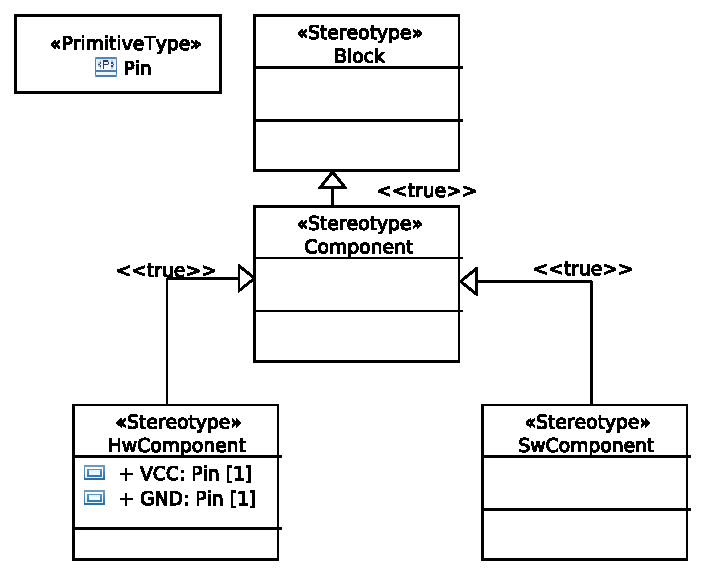
\includegraphics[width=0.6\textwidth, keepaspectratio]{img/StereotypeD}\label{fig:sysml_stereo}}
    ~\\
    \subfloat[System Block Definition Diagram]{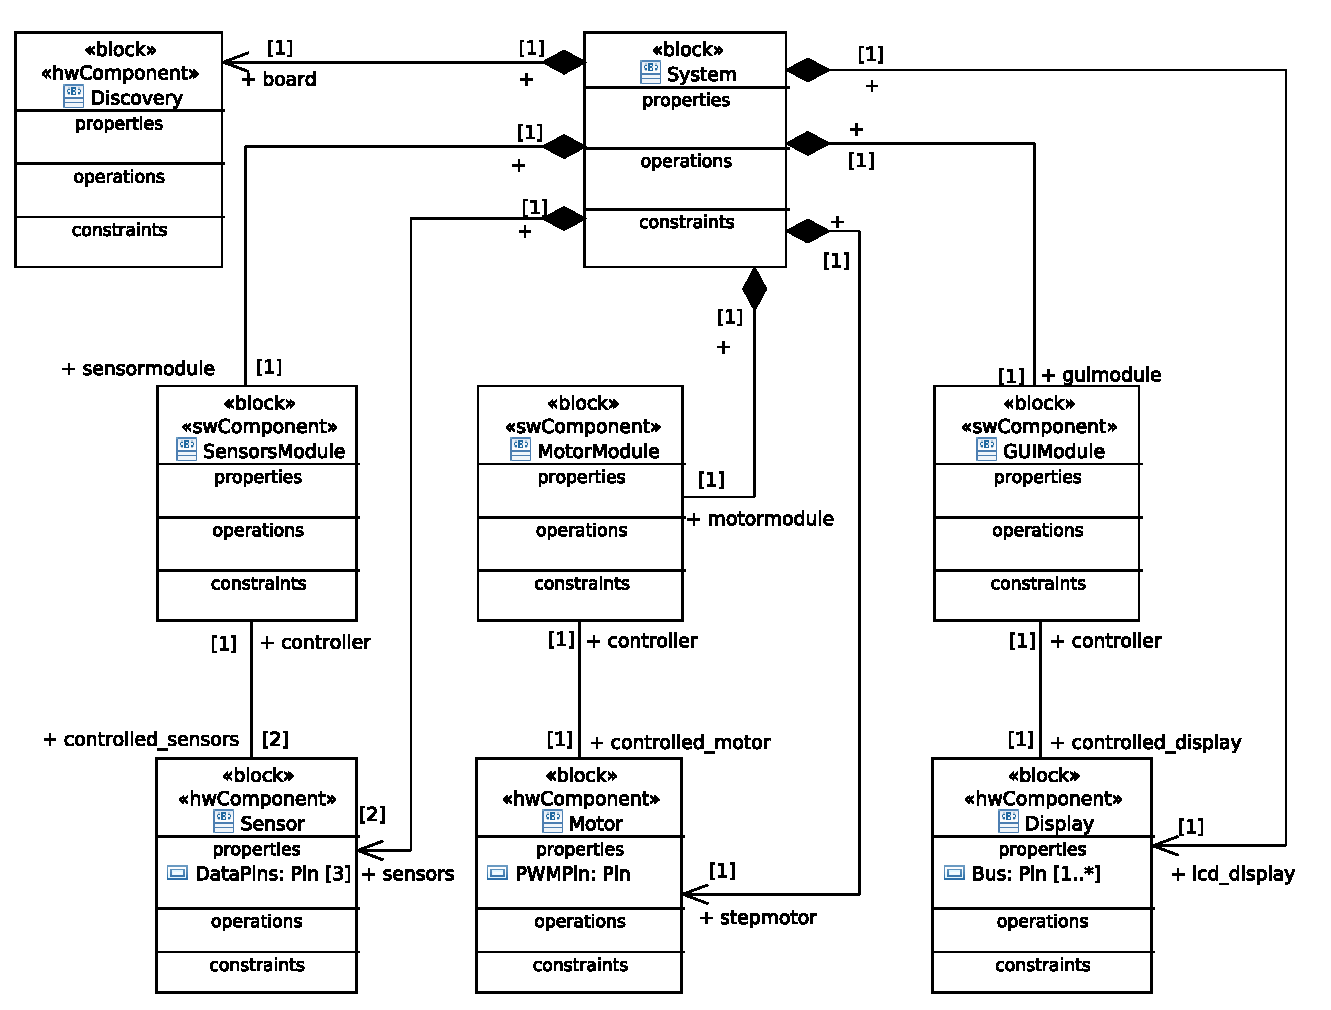
\includegraphics[width=\textwidth, keepaspectratio]{img/BlockDefinitionD}\label{fig:sysml_block}}
    \caption{System architecture shown using SysML diagrams.}\label{fig:sysml}
\end{figure}
\begin{figure}[tp]
    \ContinuedFloat
    \centering
    ~\\
    \subfloat[A bounded feasible region]{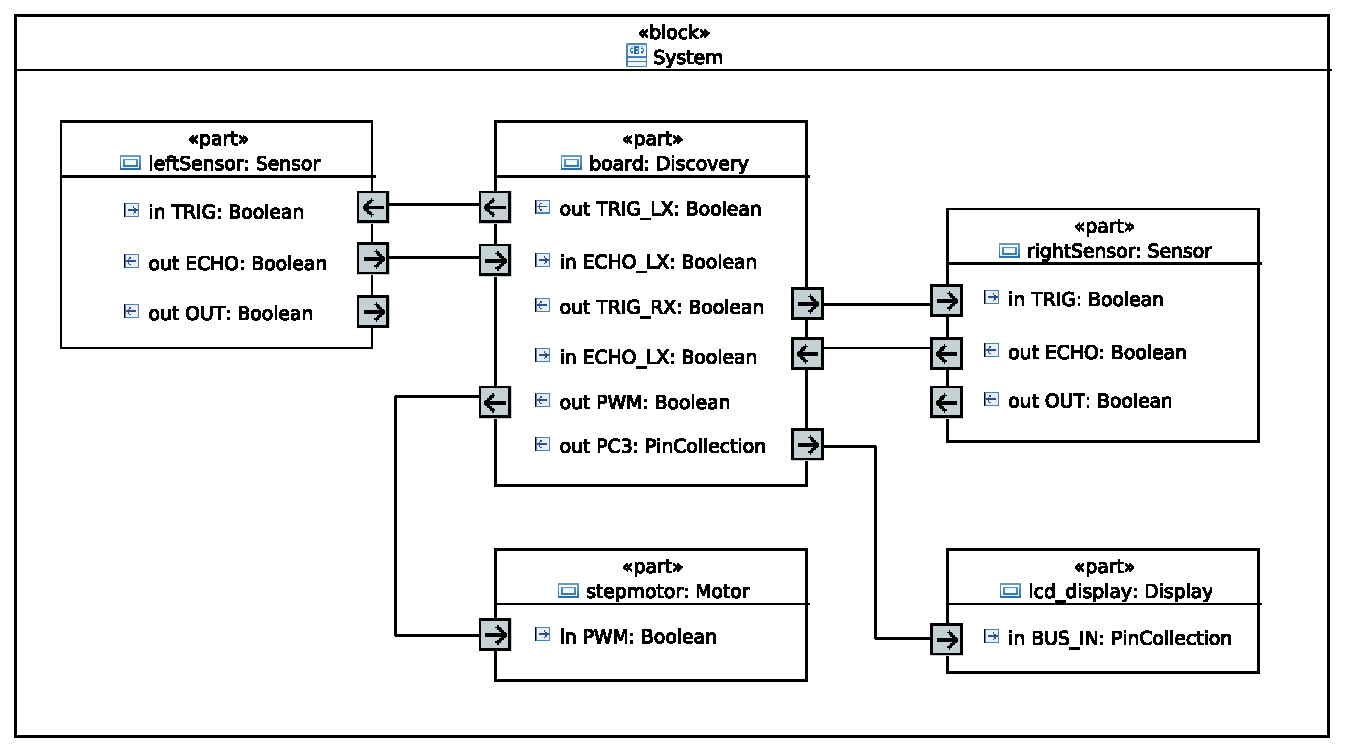
\includegraphics[width=\textwidth, keepaspectratio]{img/InternalBlockD}\label{fig:sysml_internal}}
    \caption{System architecture shown using SysML diagrams. (cont.)}
\end{figure}


\section{Hardware components}

Hardware components choice was driven by parts availability and their price per unit. We will first illustrate external hardware components, before moving on describing briefly the used microcontroller.

\subsection{Ultrasonic sensors}

To detect obstacles in front of the system two two ultrasonic distance sensors have been used. The choice fell on two \textit{HY-SRF05} sensors, shown in Figure \ref{fig:sensor}. Ultrasonic sensors overcome many of the weaknesses of IR sensors, the latter affected easily by color of obstacles and lighting of the environment. On the contrary, ultrasonic sensors provide precise distance measurement regardless of these conditions, because they use ultrasonic sound waves.

%% TODO: crop images
\begin{figure}[htp]
\centering
\hspace*{\fill}
\subfloat[Sensor's appearance]{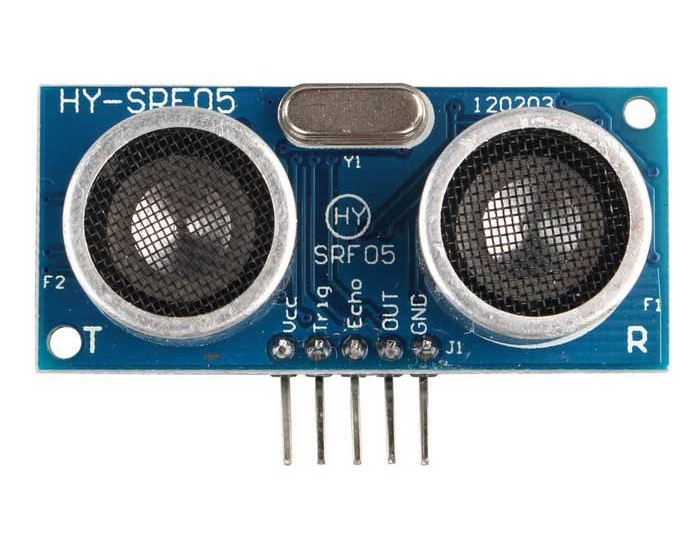
\includegraphics[width=0.4\textwidth,keepaspectratio]{img/hy-srf05.jpg}\label{fig:sensor_appearance}}
\hfill
\subfloat[Sensor's dimension]{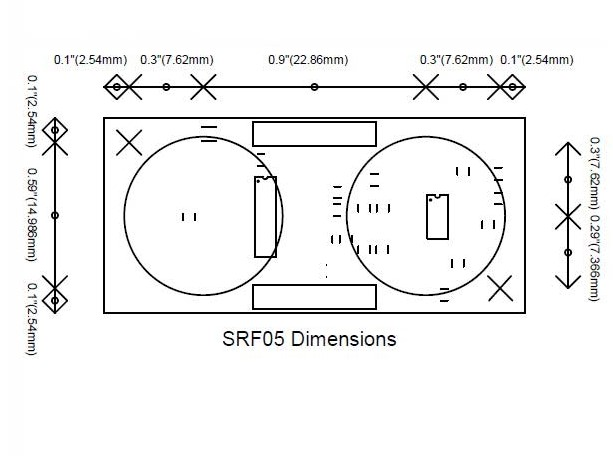
\includegraphics[width=0.5\textwidth,keepaspectratio]{img/hy-srf05-dim.jpg}\label{fig:sensor_dimensions}}
\hspace*{\fill}\\
\caption{HY-SRF05 Ultrasonic Distance Sensor.}
\label{fig:sensor}
\end{figure}

To check if an object is in the area covered by the ultrasonic sensor, it is needed to supply a pulse at least \SI{10}{\micro\second} long to the {\em trigger} input. The HY-SRF05 will send out an 8 cycle burst of ultrasound at \SI{40}{\kilo\hertz} and raise its echo line to high value. It then listens for an echo, and as soon as the sensor detects the echo it will lower down echo line value again.

The echo line is therefore a pulse whose width is exactly the time needed by the ultrasonic wave to hit an obstacle and come back to the sensor. Dividing this time by 2 times the speed of sound will give us the distance of the object. If nothing is detected then the HY-SRF05 will lower its echo line anyway after about \SI{30}{\milli\second}.





\subsection{Servo motor}

In order to change sensors' position a servo motor is used. A typical servo consists of a small electric motor driving a train of reduction gears. In particular for this work, the choice fell on HS-645MG from Hitec, shown in Figure \ref{fig:motor}.

\begin{figure}[tp]
\centering
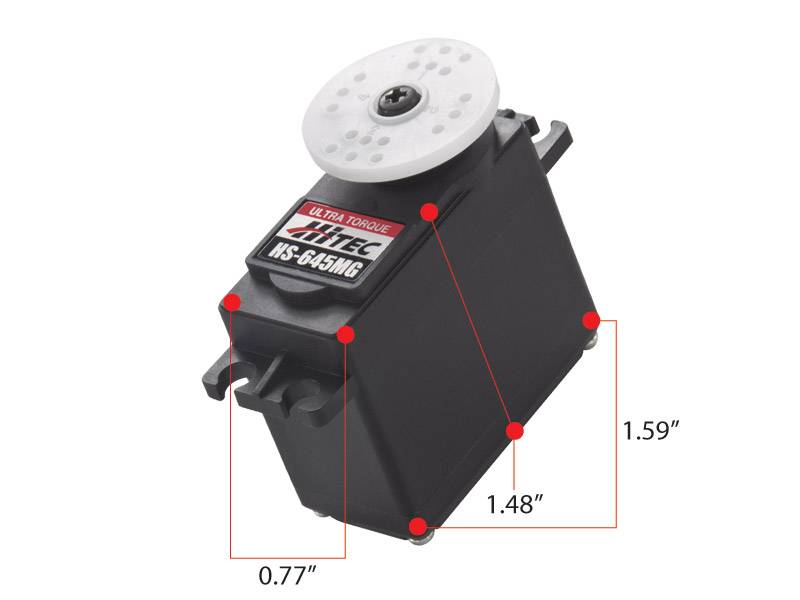
\includegraphics[width=0.6\textwidth,keepaspectratio]{img/hs-645mg.jpg}
\caption{HS-645MG servo motor}
\label{fig:motor}
\end{figure}

The servo motor will constantly check whether the position of the arm is correct with respect to the desired position, expressed as PWM signal, generating a correction torque, either clockwise or counterclockwise, in case we want to move to another position. This way the mechanical arm mounted on top of motor's shaft will move from one desired orientation angle to another.

The PWM signal used to control this servo motor expresses the desired position in terms of duration of the pulse sent at a constant frequency. To keep the motor in the same position, the same pulse must be repeated at the working frequency. Working frequency of a HS-645MG is \SI{50}{\hertz}, while minimum and maximum positions are expressed respectively by sending pulses \si{700} and \SI{2300}{\micro\second} long.


%The position of the output, measured by the potentiometer, is continually compared to the commanded position from the control. Any difference gives rise to an error signal in the appropriate direction, which drives the electric motor either forwards or backwards, and moving the output shaft to the commanded position. This kind of motors are controlled by sending an electrical pulse of variable width (PWM), through the control wire. There is a minimum pulse, a maximum pulse, and a repetition rate. The PWM sent to the motor determines position of the shaft, and based on the duration of the pulse sent via the control wire the rotor will turn to the desired position. Servos will not hold their position forever, hence the position pulse must be repeated to instruct the servo to stay in position. In the HS-645MG the repetition frequency (or working frequency) is $50Hz$ and the minimum - maximum PWM amplitude are respectively $900-2100 \mu s$

\subsection{Development board and LCD}

These devices are controlled by a STM32F4 Discovery board, which runs both controller and applicative code using ERIKA OS as real-time operating system. The Discovery Board is shown in Figure \ref{fig:board_board}. Power can be provided to the board using a standard USB Mini Type-B connector, connected to a \SI{5}{V} power supply\footnote{Power supply must not supply more than \SI{100}{\milli\ampere}.}; board includes also a voltage regulator and two buttons, respectively a reset button and a user button.

%Basically all the computation needed to drive the motor, activate/read the sensors and to display on a LCD screen are executed on a STM32F4 micro controller based on the ARM Cortex-M4F core. In particular, to provide a quick and easy way for engineers to evaluate their micro controller chips, STM built a development board. The one chosen is the STM32F4 Discovery. The power for each board is provided by a choice of the 5 V via the USB cable, or an external 5 V power supply. They can be used as output power supplies of 3 V or 5 V (current must be less than 100 mA). The board also include a voltage regulator, reset button, user button and multiple LEDs. 


\begin{figure}
\centering
\hspace*{\fill}
\subfloat[STM32F4 Discovery board]{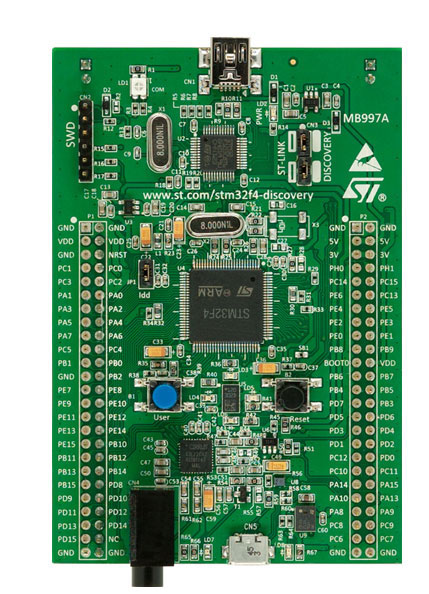
\includegraphics[width=0.34\textwidth,keepaspectratio]{img/stm32f4.jpg}\label{fig:board_board}}
\hfill
\subfloat[Expansion board for STM32F4 Discovery board]{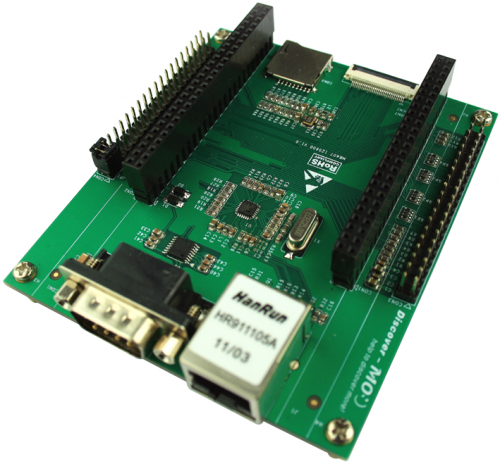
\includegraphics[width=0.34\textwidth,keepaspectratio]{img/baseboard.png}\label{fig:board_expansion}}
\hspace*{\fill}
\\
\subfloat[LCD Screen included with Expansion board kit]{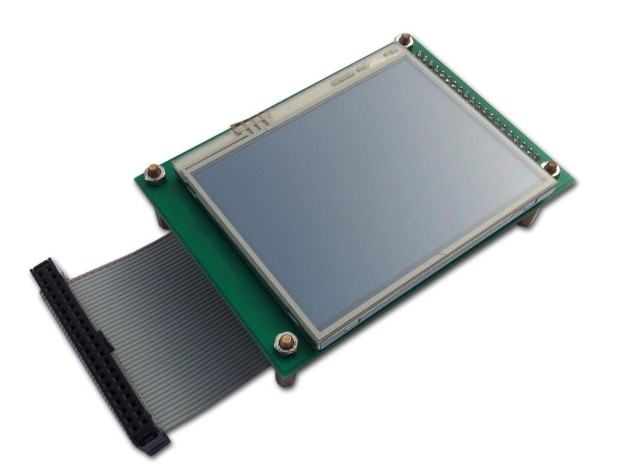
\includegraphics[width=0.6\textwidth,keepaspectratio]{img/lcd.jpg}\label{fig:board_lcd}}

\caption{STM32F4 Discovery kit}
\label{fig:board}
\end{figure}

Since the system requires a screen on which to show detected obstacles' positions, an Expansion kit was needed to connect the Discovery board to his LCD screen (STM32F4DIS-LCD). This kit includes both the LCD screen and an Expansion board (STM32F4DIS-EXT), which expands basic functionalities of the Discovery board providing additional connectors (like Ethernet and serial ones), a MicroSD card slot and connectors for LCD or camera peripherals. Expansion board and its LCD screen are both shown in Figure \ref{fig:board}.


% In order to use the LCD screen (STM32F4DIS-LCD) an expansion board is needed. The expansion board STM32F4DIS-EXT expands the functionality of the STM32F4 Discovery providing a microSD card slot, ethernet connectivity and extension connectors for LCD or camera boards.


\section{Connections and wiring}

External peripherals have been connected to the board using a small circuit obtained from a small perforated board. We will illustrate each peripheral pin and wiring scheme in following sections, while full wiring scheme can be found in Figure \ref{fig:wire_scheme}.

\begin{figure}[htp]
\centering
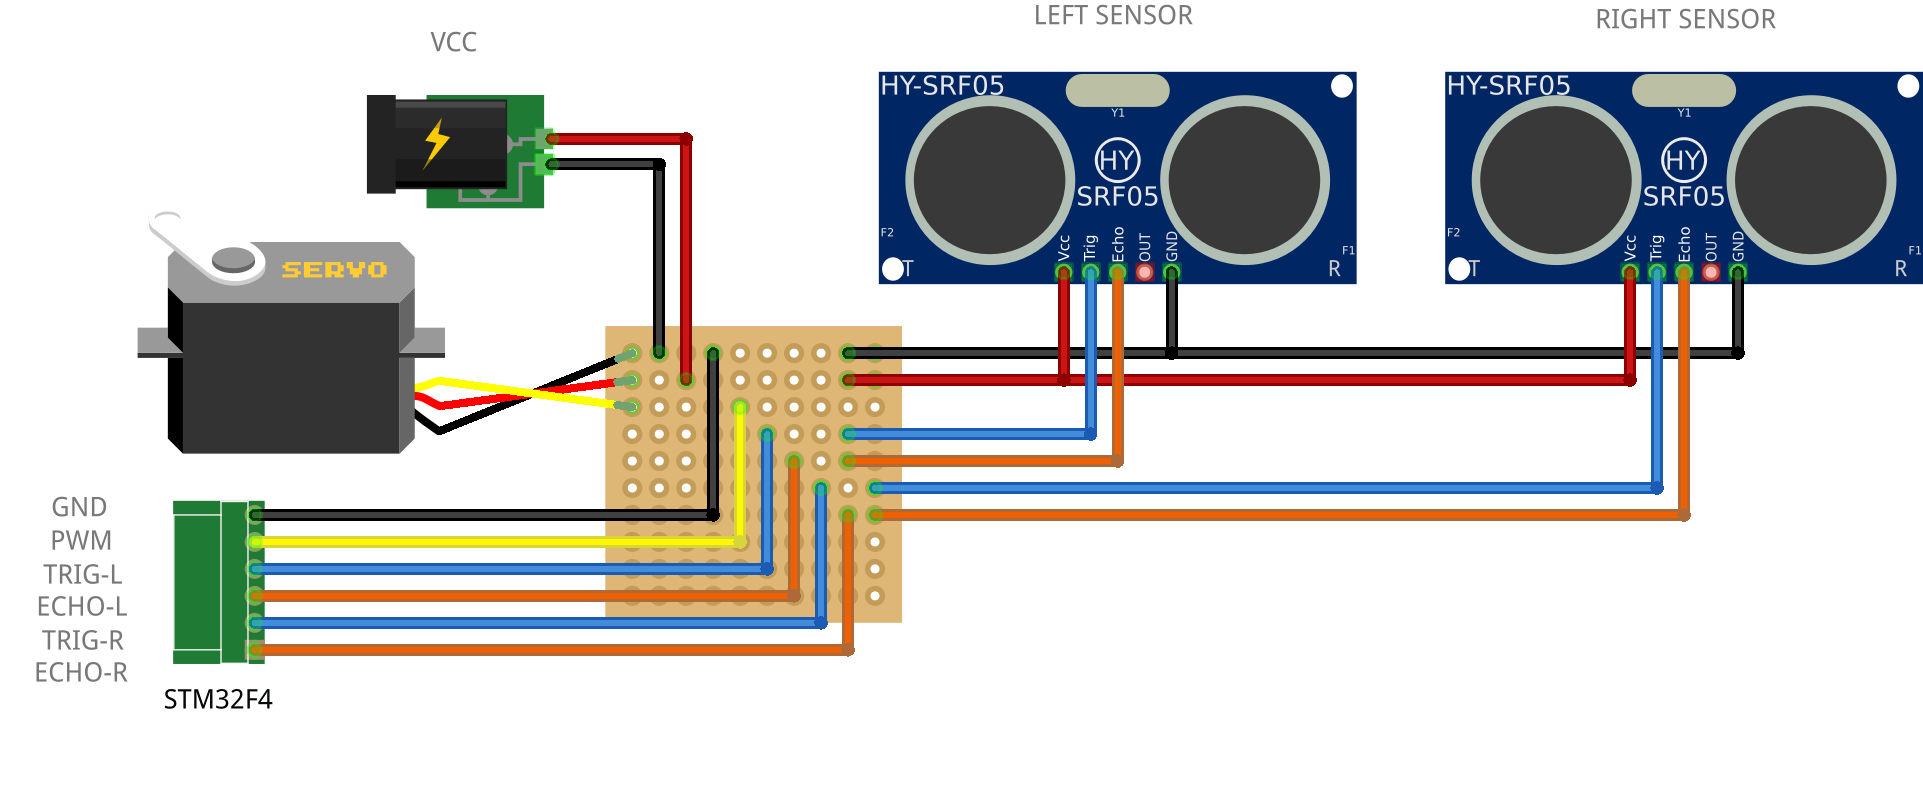
\includegraphics[width=0.8\textwidth, keepaspectratio]{img/wire-schema.png}
\caption{Full wiring scheme between external peripherals and the Discovery board}
\label{fig:wire_scheme}
\end{figure}



\subsection{Servo motor connection}
Hitec servomotors come with a universal connector called ``S'' connector. Meanings of individual wires in this connector are shown in Table \ref{tab:wire_motor}. The Discovery board has been connected to appropriate right connectors adopting the wiring scheme shown in Figure \ref{fig:wire_motor}. The PWM signal has been provided using the port and pin assigned to PWM output, as declared in Table \ref{tab:func_data_dictionary}.

%All of our Hitec servos come with the “S” or universal connector. The yellow cable is used to drive the motor with a PWM signal generated by the STM32F4 discovery board. The red and the black cable are respectively the VCC and the GND of the motor.

\begin{table}[p]
\centering

\begin{tabular}{c|c|c}
\hline
\textbf{Name} & \textbf{Cable color} & \textbf{Description}    \\ \hline
SIGNAL        & Yellow               & PWM signal to the motor \\
VCC           & Red                  & Electricity supply      \\
GND           & Black                & Ground                 
\end{tabular}
\caption{Servo motor ``S'' connector pin meanings}
\label{tab:wire_motor}
\end{table}

\begin{figure}[p]
\centering
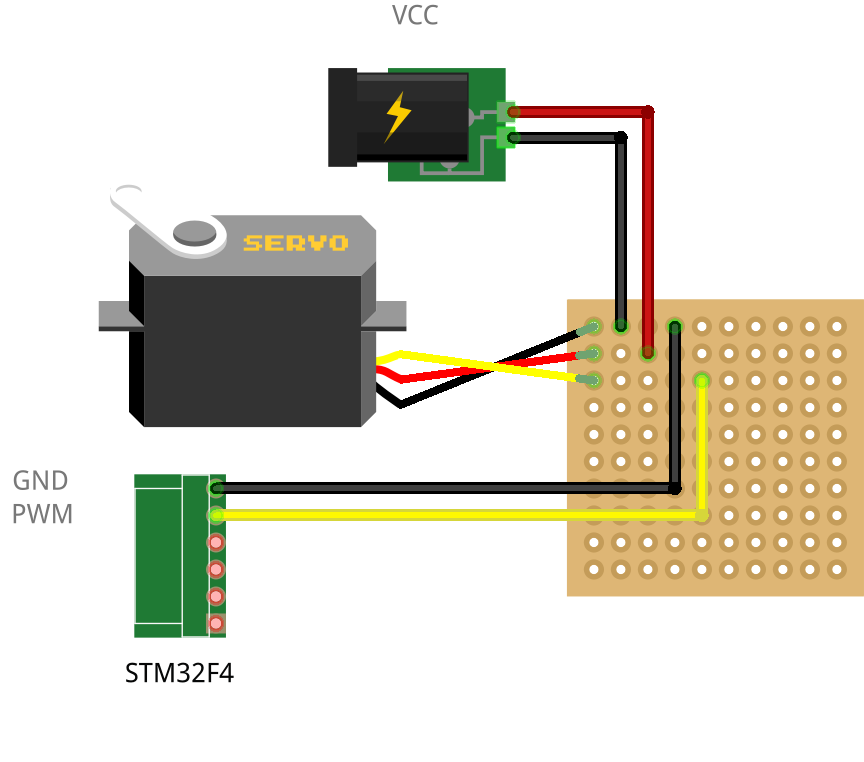
\includegraphics[width=0.7\textwidth,keepaspectratio]{img/wire-servo.png}
\caption{Servo motor wiring scheme}
\label{fig:wire_motor}
\end{figure}




\subsection{Ultrasonic sensors connection}

HY-SRF05 sensors have 5 pins, whose meanings are shown in Table \ref{tab:wire_sensor}. These sensors can be used in two different configurations, wither using one pin both for trigger/echo or 2 separate pins. The 2 pins mode is the default one and can be selected by simply leaving the OUT pin unconnected. The Discovery board has been connected to right pins adopting the wiring scheme shown in Figure \ref{fig:wire_sensor}. Each sensors' pin has been connected to the relative board one, as declared in Table \ref{tab:func_data_dictionary}. 

% Hence, VCC PIN is connected to the electricity supply (5V), the GND PIN is connected to the ground, the OUT PIN is leaved unconnected and the Trig PIN/Echo PIN are connected separately to the board.

\begin{table}[p]
\centering
\begin{tabular}{c|c}
\hline
\textbf{Pin} & \textbf{Description}                         \\ \hline
VCC          & Power supply                                 \\
TRIG         & \SI{10}{\micro\second} pulse trigger input   \\
ECHO         & Sensor response                              \\
OUT          & Change sensor mode                           \\
GND          & Ground                  
\end{tabular}
\caption{Ultrasonic sensors connection}
\label{tab:wire_sensor}
\end{table}

\begin{figure}[p]
\centering
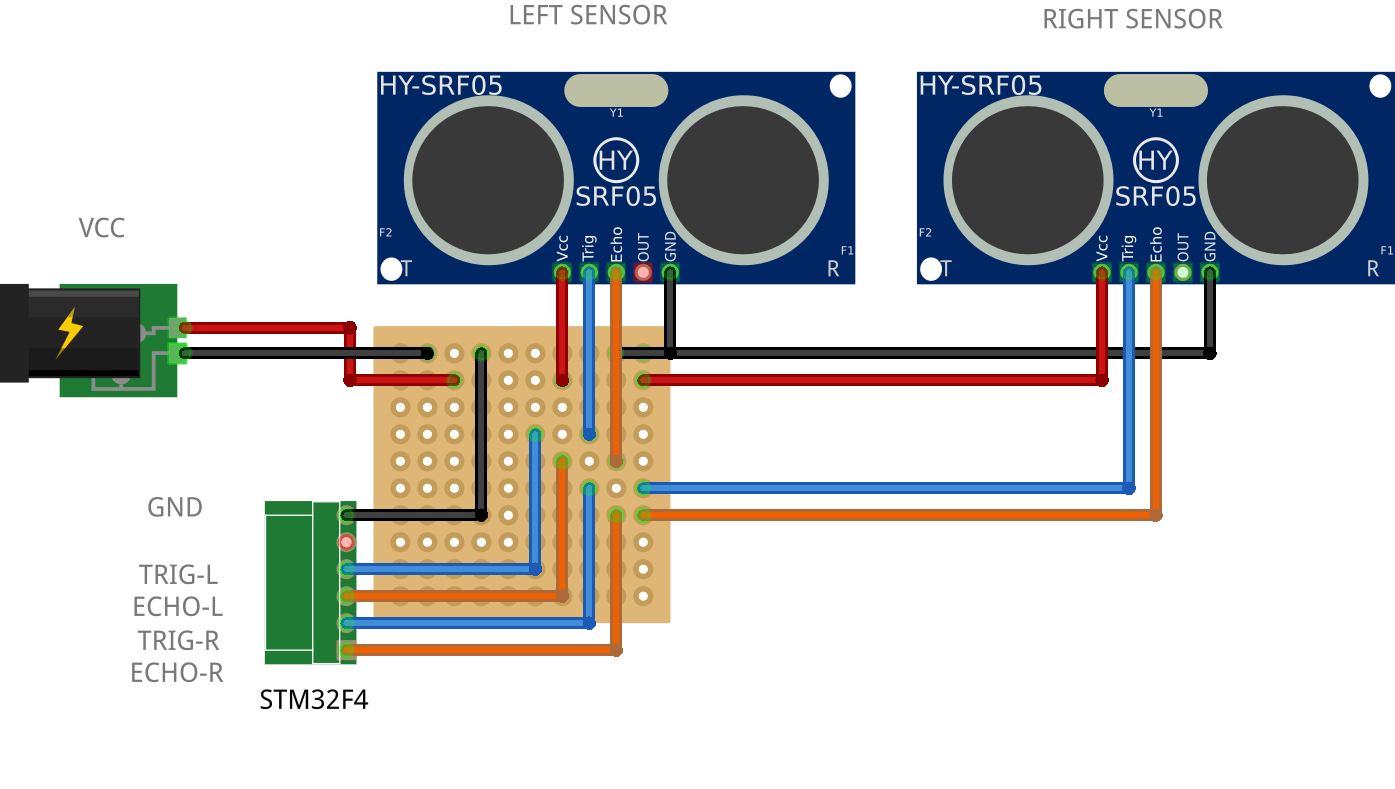
\includegraphics[width=0.8\textwidth, keepaspectratio]{img/wire-sensors.png}
\caption{Ultrasonic sensor wiring scheme}
\label{fig:wire_sensor}
\end{figure}

\begin{figure}[p]
\centering
\includegraphics[width=0.8\textwidth, keepaspectratio]{img/Sonar.png}
\caption{Appearance of the final system.}
\label{fig:sonar}
\end{figure}





\chapter{Software implementation}


%An embedded system is a special-purpose computer system designed to perform one or a few dedicated functions, sometimes with real-time computing constraints. Hence, developing software for an embedded system is one of the most critical phase of the design of the entire system. Furthermore meet some real-time constraint it's not easy without some analysis. Developing real-time software requires additional special care, due to the extra time dimension. An error occurring in a particular state may not occur again by restarting the system in the same state, since time is different. Design time in not wasted, but invested in the future.
% Si parla del processo a V? Abbiamo usato un bottom-up approach?

We will now show briefly software organization, highlighting major features provided by each of its components.



\section{RTOS and API}

Since this system has to deal with real-time requirements, a real-time operating system (RTOS) is needed to ensure the fulfillment of these requirements. To this, we used Erika Enterprise RTOS, which provides support to fixed and dynamic priority scheduling, priority ceiling and so on.

Erika OS is a modular and incremental operating system, OSEK/VDX standard compatible, which can be compiled in such a way it provides only needed resources and primitives, hence reducing his already small flash memory footprint.

System requirements could be accomplished by simply including only fixed priority scheduling support, hence we used the smallest-footprint version available to implement system's controller, including only needed ST libraries. In addition to ST provided libraries, we included some other higher-level libraries, to manage respectively servo motor and input/output pins.


%In order to meet all the deadlines and make the system work correctly, an RTOS has mounted on the STM32F4 board. In particular it is used Erika Enteprise that is an open-source OSEK/VDX Hard Real Time Operating System. Erika OS provide an hard real-time support with fixed priority scheduling and immediate priority ceiling. Furthermore provide also support for earliest deadline first (EDF) and resource reservation schedulers. One of the most important feature of Erika is that can be used in an sort of "incremental way" including or excluding at flash time some libraries. Using this way of reasoning, the footprint of Erika on main flash of microcontroller is only 1-4 Kb, hence suitable for 8 to 32 bit microcontrollers. Last but not least, Erika can be flashed and configured easily  using RT-Druid with Eclipse plugins.
% Scriviamo qualcosa sulle lib di Tilen? No, già detto un minimo

\section{Software components}

In this section we will illustrate application and control software organization.

\subsection{Main module and tasks}

Main module is in charge of coordinating all other modules. It handles {\em SysTick} timer interrupts and manages the three concurrent real-time tasks that compose the system:

\begin{description}
    \item[GUI Task] executed with a period of \SI{90}{\milli\second}, it checks whether the user has pressed B\_ZOOM and refreshes the LCD screen.
    \item[Step Task] executed with a period of \SI{70}{\milli\second}, it sends the trigger pulse to both sensors and reads previously detected distance, moving then the motor to the next desired position.
    \item[Stop Trigger Task]  executed with the same period of Step Task, but with a different phase, it simply stops sending the trigger signal to both sensors.
\end{description}


\subsection{Motor module}

Motor module is in charge of handling all servo motor routines and control, hence taking care of PWM generation, motor state and so on. This is all transparent to other modules, which can only see the following interface. In the code, we refer to user-domain positions as the positions as they are perceived by the user. The library converts automatically all provided positions in user-domain in motor-domain positions (i.e. width of PWM pulse).

% The motor library permit to control easily the servo motor without take care of modulating the PWM. A simple data struct contains data of the motor. An example of function implemented can be found in code snippet below.

\begin{minted}{c}
/*
 * Returns the user range domain motor position.
 * in:  void
 * ret: int_t, motor position in user range domain
 */
extern int_t motor_get_pos();

/*
 * Initializes motor with initial parameters.
 * in:  initial motor position
 *      initial motor direction%*      default motor increment % What?
 * ret: void
 */
extern void motor_init(int_t init_pos, direction_t init_dir);

/*
 * Sets position of the motor and moves the motor to chosen position
 * in:  new position of the motor
 * ret: void
 */
extern void motor_set_pos(int_t position);

/*
 * Sets a new value for the direction of the motor movement
 * in:  new value for the direction
 * ret: void
 */
extern void motor_set_dir(direction_t direction);

/*
 * Moves the motor following the current increment and direction
 * in:  void
 * ret: void
 */
extern void motor_step();
\end{minted}


\subsection{GUI module}

LCD screen handling and refresh is taken care by GUI module. This module uses a custom defined library to refresh ``widgets'' content on the screen. Screen content changes between different modes:
\begin{description}
    \item[Calibration Mode] In this mode a message is printed on the screen telling the user to move the mechanical arm in the desired orientation.
    \item[Scanning Mode] In this mode it will be shown background in Figure \ref{fig:background}, over which current zoom level, maximum distance and obstacles positions will be drawn, according to what has been specified in {\em User Requirements}.
\end{description}

The GUI module interface is the following:

%All the things that regards the LCD screen and in general the graphical user interface of the system is managed by the GUI library. In the code snippet below some example of function realized can be found.

\begin{figure}[tp]
\centering
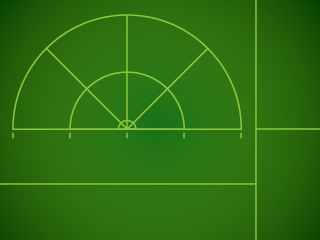
\includegraphics[width=0.6\textwidth, keepaspectratio]{img/background-with-interface.png}
\caption{LCD main background}
\label{fig:background}
\end{figure}

\begin{minted}{c}
/*
 * Changes zoom level to the next one, starting back from zero if
 * maximum zoom level is reached.
 * in:  void
 * ret: void
 */
extern void gui_change_zoom_level();

/*
 * Sets current position and distance that has been measured.
 * in:  void
 * ret: void
 */
extern void gui_set_position(int_t pos, int_t distance);

/*
 * Shows on the screen the calibration message.
 * in:  void
 * ret: void
 */
extern void gui_show_calibration_message();

/*
 * Initializes the interface for Scanning mode with all static
 * texts and background.
 * in:  void
 * ret: void
 */
extern void gui_interface_init();

/*
 * Refreshes LCD screen, to be called only in Scanning mode after
 * gui_interface_init call.
 * in:  void
 * ret: void
 */
extern void gui_refresh();
\end{minted}

\subsection{Sensor module}

Sensor module handles all sensor pins and states, requiring main module to call some methods at specified intervals. In particular, this module expects a file called \path{constants.h} in which it is defined a \mintinline{c}{SYST_PERIOD} constant, expressing {\em SysTick} period in microseconds. This because \mintinline{c}{sensor_read} function shall be called every \mintinline{c}{SYST_PERIOD} \si{\micro\second} for distances to be returned correctly by this module.

Module interface is the following:

% Another library developed is the sensor library. It realize the function needed to trigger the sensors, read the response and calculate the distance. An example of the implemented function can be found in the code snippet below.

\begin{minted}{c}
/* 
 * Initializes all sensors' pins and ports
 * in:  void
 * ret: void
 */
extern void sensors_init();

/*
 * Reads both sensors value, to be called each SYST_PERIOD microseconds
 * to obtain valid measured distances in centimeters.
 * in:  void
 * ret: void
 */
extern void sensors_read();

/*
 * Sends trigger signal, raising trigger line of both sensors.
 * At the moment of sending the trigger pulse it also updates the
 * global calculated distance at the previous step.
 * in:  void
 * ret: void
 */
extern void sensors_send_trigger();

/*
 * Stops trigger signal, lowering down both lines.
 * in:  void
 * ret: void
 */
extern void sensors_stop_trigger();

/*
 * Returns the last calculated distance.
 * in:  void
 * ret: int_t, the last calculated distance
 */
extern int_t sensors_get_last_distance();
\end{minted}




\chapter{Testing}

%Testing is a fundamental phase in the developing process of an embedded system. It is important to define test plan at each level of design and is necessary to test not only the software but also if the global system matches all the specified requirements.

We will now show a subset of all tests that have been performed on the system. 

Through all phases of system development, several tests have been performed, either on hardware or software components, which involved both prototypes and final system implementation. Main tests on the system involved real use case scenarios, e.g.\ observing system's reactions to obstacles in sonar's field of vision at different distances and angles, providing hence the system a various set of different inputs.

Apart from these tests, individual software components have also been tested using {\em CUnit} suite, performing functional and conformance testing. According to what is required by the committee, only these latter tests are illustrated in following sections.


\section{Conformance Tests}

This section illustrates tests performed by the first suite included in our automatic testing program. This suite performs conformance testing of a state machine that is included inside Sensor module used to manage erroneous states the system can get into after partial or total hardware failures. These erroneous states are all identified depending on each sensor's echo response width, as shown in Figure \ref{fig:echo_widths}. In the Figure, arrows represent two consecutive activations of Step Task.






\begin{figure}[tp]
\centering
\subfloat[Correct sensor behavior, next state will be State OK and trigger signal can be sent again at next activation]{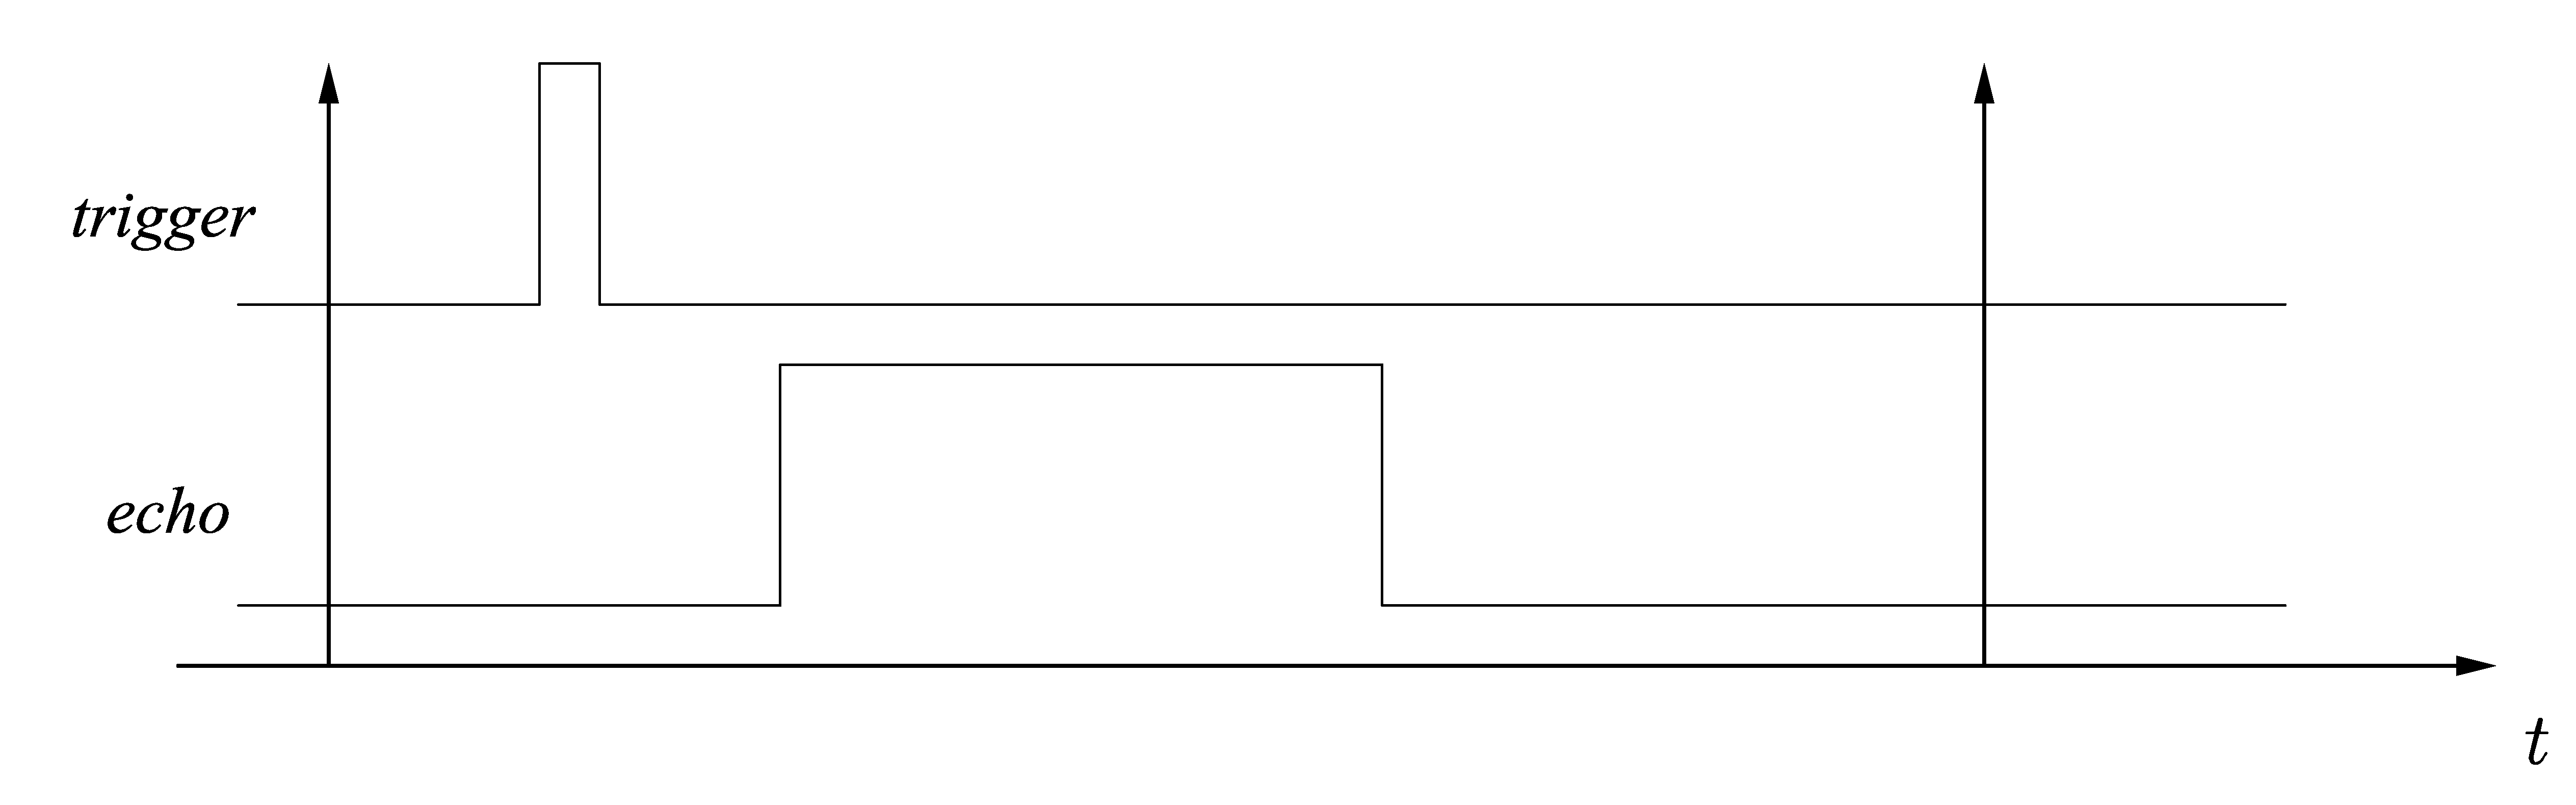
\includegraphics[width=0.8\textwidth]{tikz_img/trig_echo_ok.eps}\label{fig:state_ok}}\\

\subfloat[Stuck at zero echo behavior, next state will be State Lost and trigger signal can be sent again at next activation]{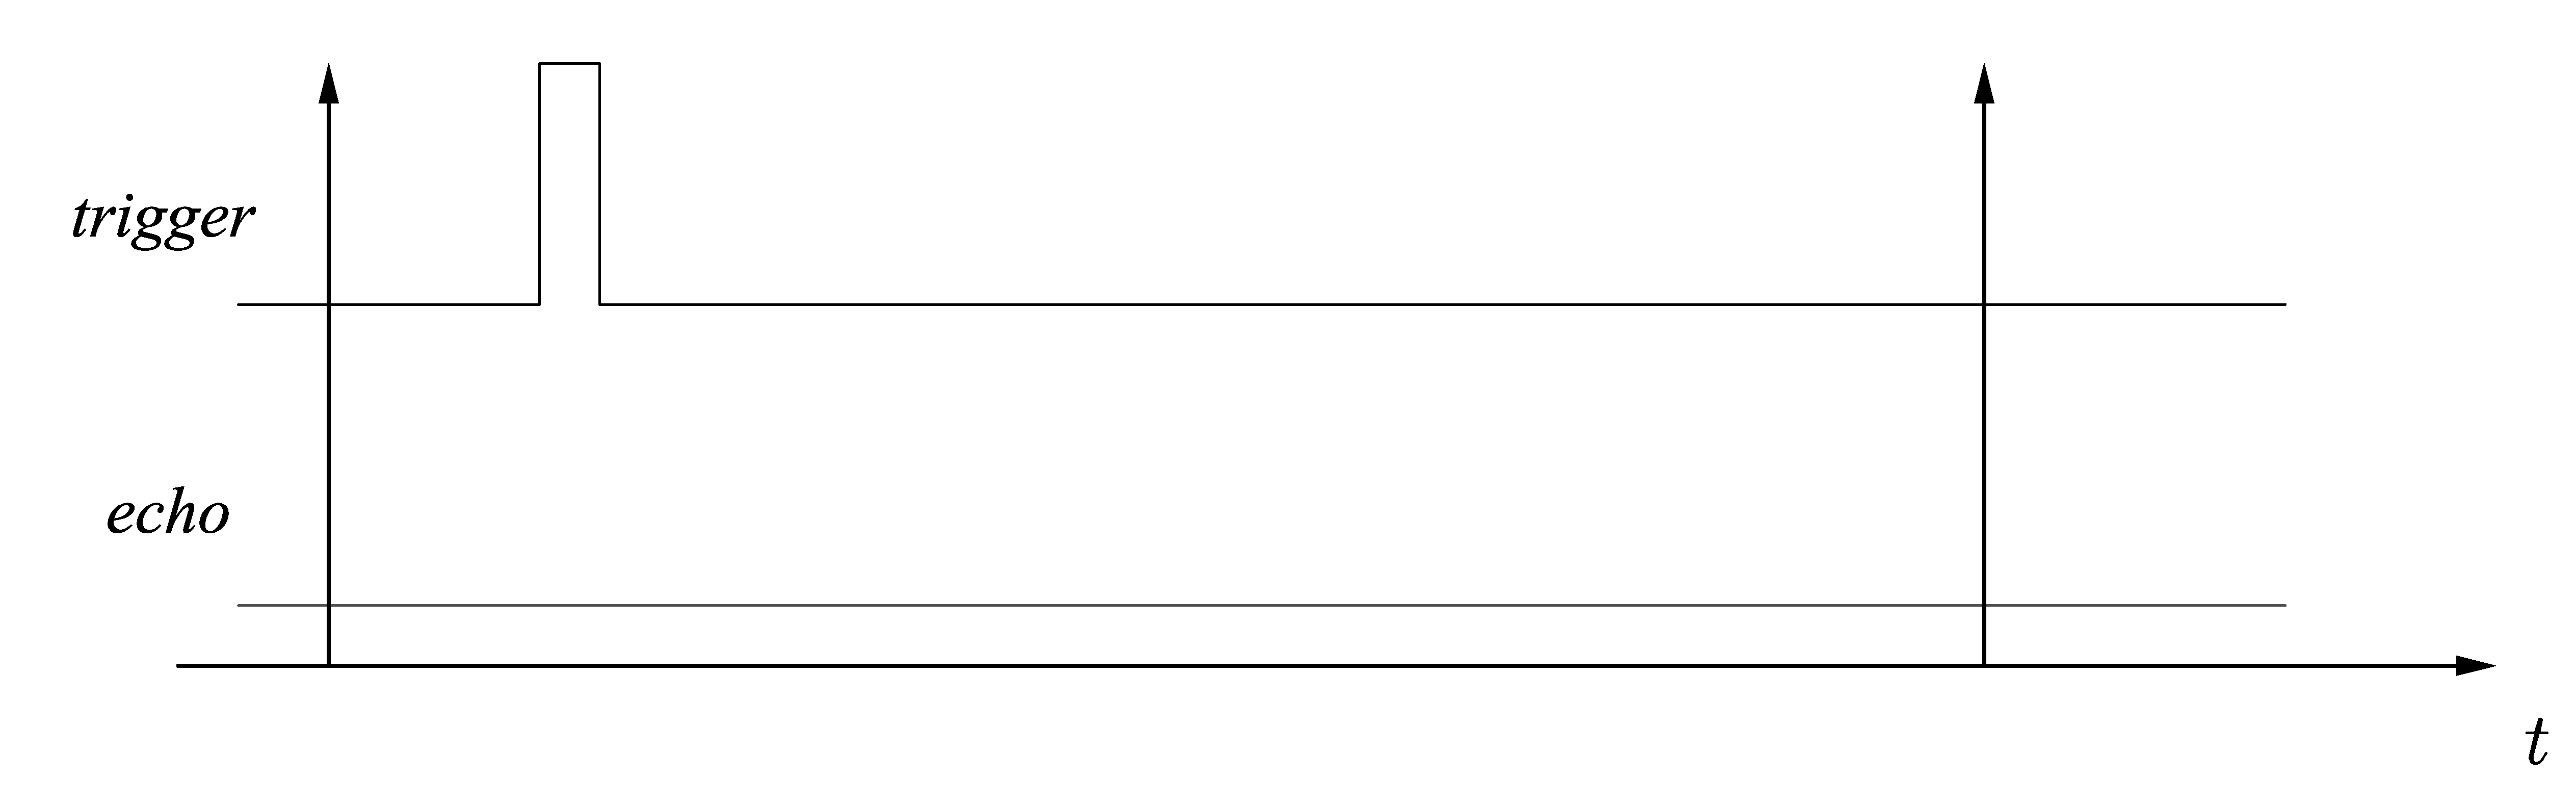
\includegraphics[width=0.8\textwidth]{tikz_img/trig_echo_lost.eps}\label{fig:state_lost}}\\

\subfloat[Stuck at one echo behavior, next state will be State Long and trigger signal will not be sent at next activation]{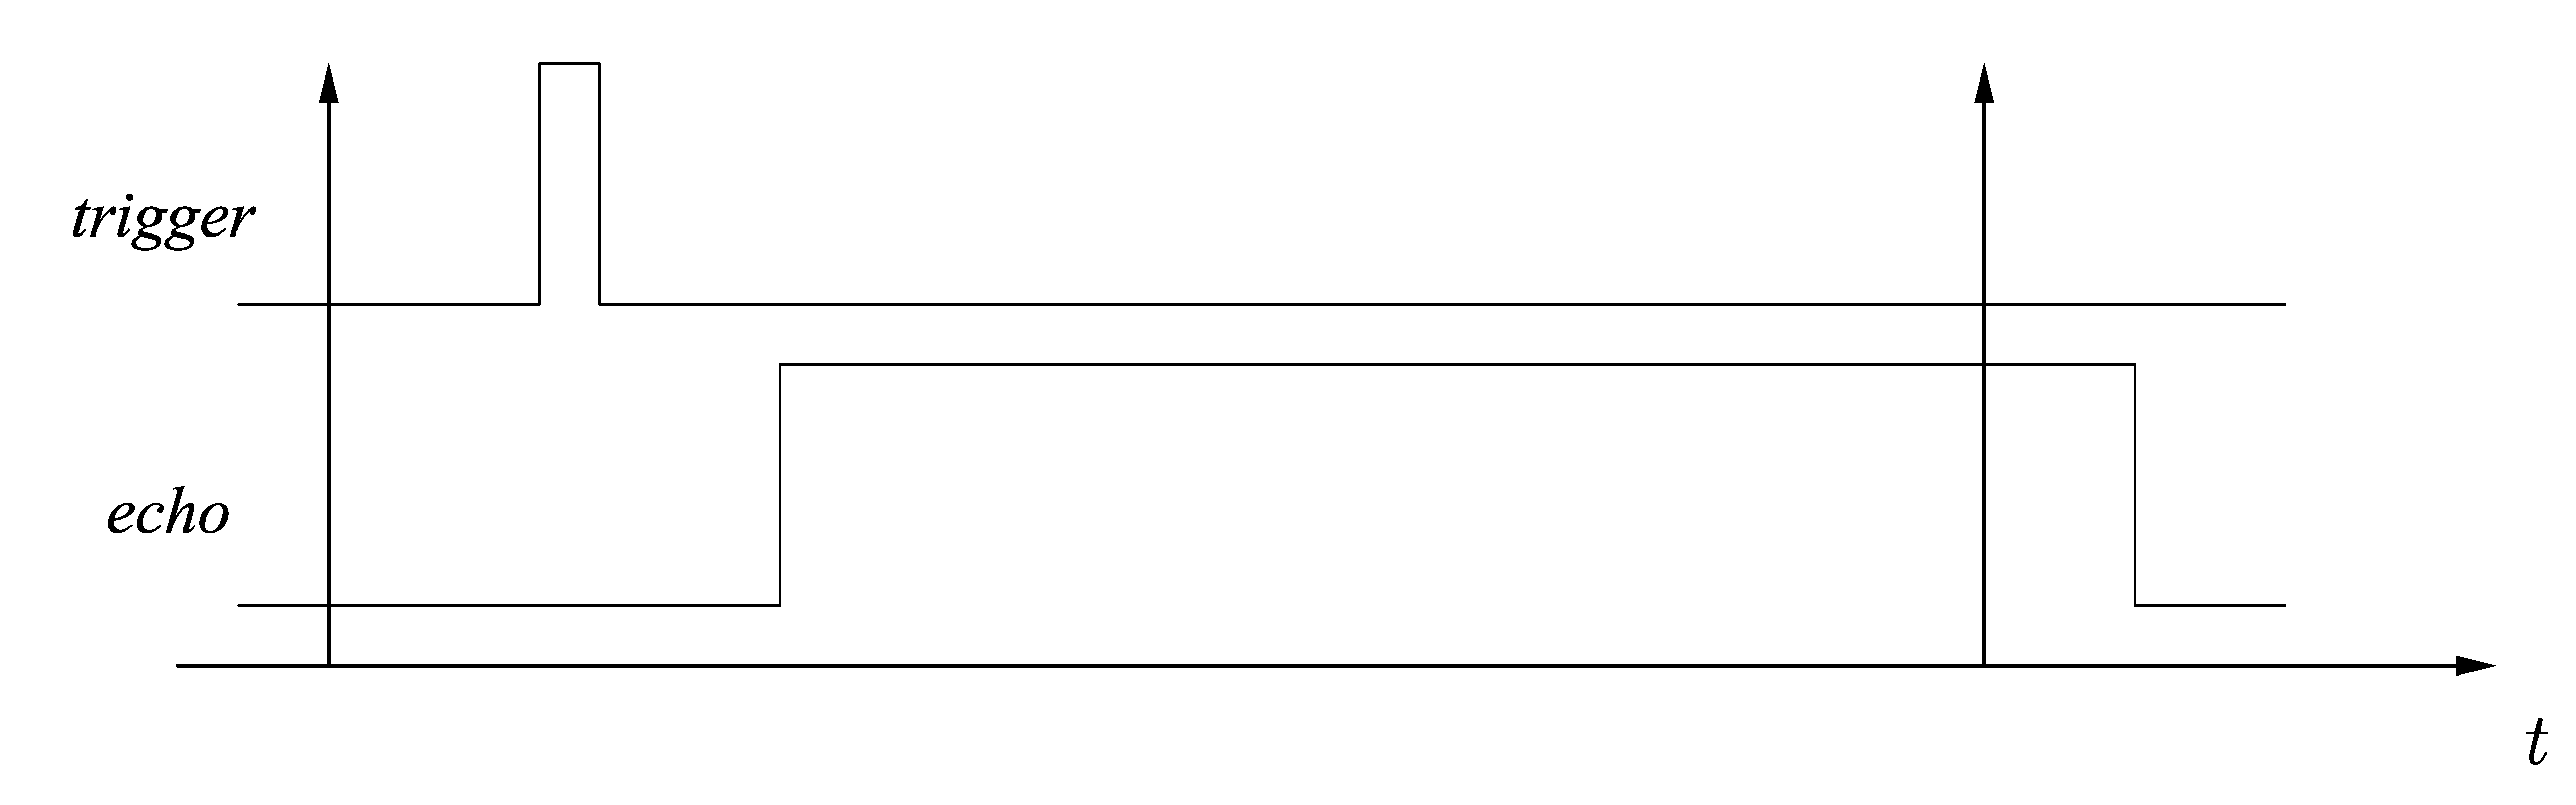
\includegraphics[width=0.8\textwidth]{tikz_img/trig_echo_long.eps}\label{fig:state_long}}\\

\subfloat[Termination of a stuck at one behavior, next state will be State Next OK and trigger signal can be sent again at next activation]{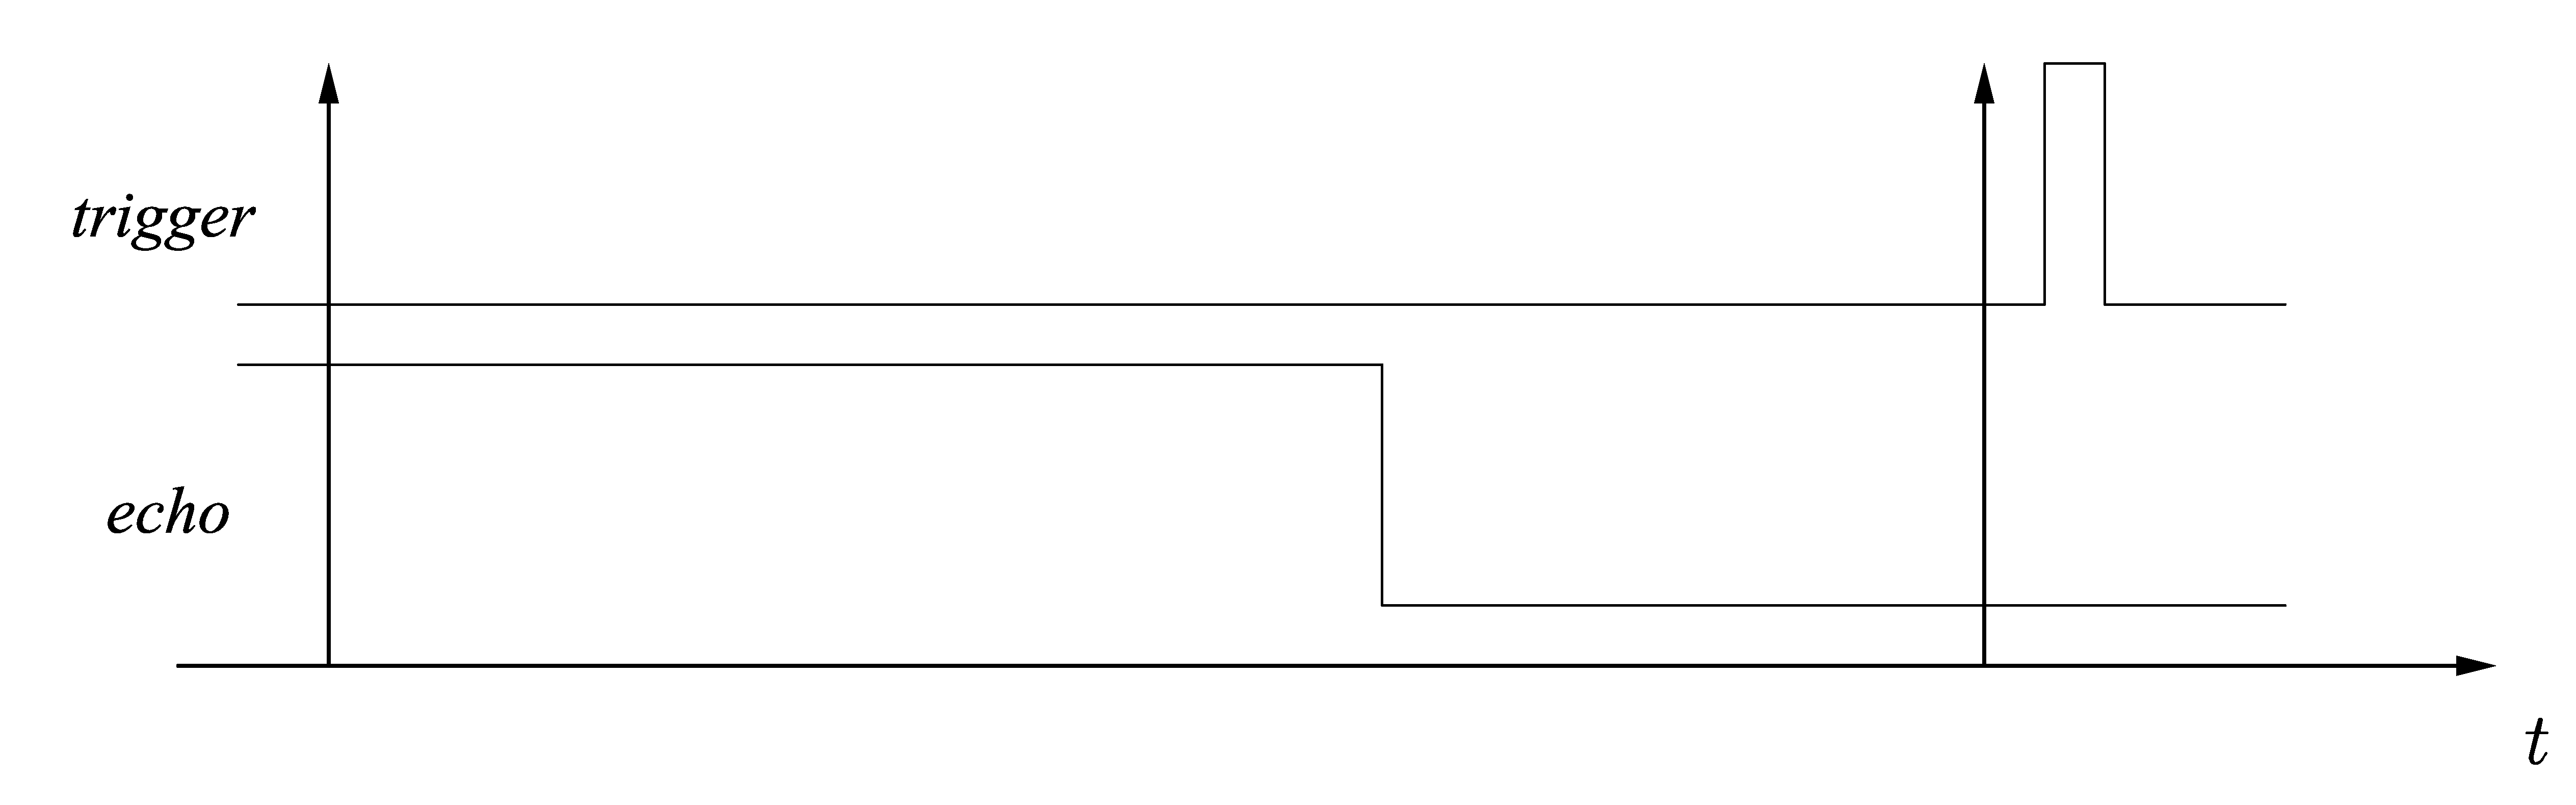
\includegraphics[width=0.8\textwidth]{tikz_img/trig_echo_next_ok.eps}\label{fig:state_next_ok}}\\
\caption{Various conditions that can be identified by listening to a sensor's echo signal.}
\label{fig:echo_widths}
\end{figure}




Starting from this, possible states in which a system can transition to are:
\begin{description}
    \item[State OK] if echo correctly started and finished within Step Task period;
    \item[State Lost] if echo did not start at all within current period;
    \item[State Long] if echo started within current period, but did not finished;
    \item[State Next OK] if echo started within (one or more) previous period(s), but finished during current period.
\end{description}

When no reply or a too long reply are detected by the system the detected distance is not valid and cannot be shown to the user. Probably a hardware failure made the line getting stuck at either 0 or 1 value. Otherwise, the detected distance is valid.

Obviously, Step Task period must be set in such a way valid distances are not wrongly interpreted as too long ones. To do so, various testings have been made, obtaining the optimal trade-off.

Notice that in the case a sensor's echo line is stuck at a high value, no trigger signal is sent to the sensor, to avoid overlapping of multiple responses altogether. Trigger signals will start to be sent again after the line changes its value again.

The resulting state machine is the one shown in Figure \ref{fig:state_machine}, where for the sake of clarity of the scheme states, inputs and outputs have been translated into integer values. Translation table can be found in Table \ref{tab:state_table}.

\begin{figure}[tp]
\centering
%% MACCHINA A STATI

\begin{tikzpicture}[scale=0.2]
\tikzstyle{every node}+=[inner sep=0pt]
\draw [black] (39.9,-27.9) circle (3);
\draw (39.9,-27.9) node {$0$};
\draw [black] (20.5,-16.1) circle (3);
\draw (20.5,-16.1) node {$1$};
\draw [black] (20.5,-41.8) circle (3);
\draw (20.5,-41.8) node {$2$};
\draw [black] (62.5,-41.8) circle (3);
\draw (62.5,-41.8) node {$3$};
\draw [black] (37.34,-26.34) -- (23.06,-17.66);
\fill [black] (23.06,-17.66) -- (23.49,-18.5) -- (24.01,-17.65);
\draw (32.48,-21.5) node [above] {$3\mbox{ }/\mbox{ }1$};
\draw [black] (43.9,-23.2) -- (41.84,-25.62);
\draw (46.3,-22.71) node [above] {$reset$};
\fill [black] (41.84,-25.62) -- (42.74,-25.33) -- (41.98,-24.68);
\draw [black] (17.573,-15.499) arc (286.12502:-1.87498:2.25);
\draw (14.6,-10.54) node [left] {$3\mbox{ }/\mbox{ }1$};
\fill [black] (19.2,-13.41) -- (19.45,-12.5) -- (18.49,-12.78);
\draw [black] (42.46,-29.47) -- (59.94,-40.23);
\fill [black] (59.94,-40.23) -- (59.53,-39.38) -- (59,-40.24);
\draw (48.17,-35.35) node [below] {$0,1\mbox{ }/\mbox{ }0$};
\draw [black] (42.785,-27.093) arc (100.50277:16.31052:16.754);
\fill [black] (42.79,-27.09) -- (43.66,-27.44) -- (43.48,-26.46);
\draw (57.64,-28.79) node [above] {$2,3\mbox{ }/\mbox{ }1$};
\draw [black] (37.46,-29.65) -- (22.94,-40.05);
\fill [black] (22.94,-40.05) -- (23.88,-39.99) -- (23.3,-39.18);
\draw (32.48,-35.35) node [below] {$2\mbox{ }/\mbox{ }1$};
\draw [black] (22.887,-14.285) arc (123.93206:-6.85738:25.881);
\fill [black] (63.03,-38.85) -- (63.62,-38.11) -- (62.63,-37.99);
\draw (53.87,-13.18) node [above] {$0,1\mbox{ }/\mbox{ }0$};
\draw [black] (23.5,-41.8) -- (59.5,-41.8);
\fill [black] (59.5,-41.8) -- (58.7,-41.3) -- (58.7,-42.3);
\draw (41.5,-42.3) node [below] {$0,1\mbox{ }/\mbox{ }0$};
\draw [black] (21.823,-44.48) arc (54:-234:2.25);
\draw (20.5,-49.05) node [below] {$2\mbox{ }/\mbox{ }1$};
\fill [black] (19.18,-44.48) -- (18.3,-44.83) -- (19.11,-45.42);
\draw [black] (18.317,-39.748) arc (-138.50059:-221.49941:16.296);
\fill [black] (18.32,-18.15) -- (17.41,-18.42) -- (18.16,-19.08);
\draw (13.73,-28.95) node [left] {$3\mbox{ }/\mbox{ }1$};
\draw [black] (20.5,-19.1) -- (20.5,-38.8);
\fill [black] (20.5,-38.8) -- (21,-38) -- (20,-38);
\draw (20,-28.95) node [left] {$2\mbox{ }/\mbox{ }1$};
\draw [black] (63.823,-44.48) arc (54:-234:2.25);
\draw (62.5,-49.05) node [below] {$0,1\mbox{ }/\mbox{ }0$};
\fill [black] (61.18,-44.48) -- (60.3,-44.83) -- (61.11,-45.42);
\end{tikzpicture}    
\caption{Erroneous states' state machine}
\label{fig:state_machine}
\end{figure}

\begin{table}[tp]
\centering

\subfloat[States translation table]{%
\begin{tabular}{l|c}%
\hline%
\multicolumn{1}{c|}{\textbf{State Id}} & \textbf{State Label} \\ \hline%
State NEXT OK                          & 0                    \\ %
State OK                               & 1                    \\ %
State LOST                             & 2                    \\ %
State LONG                             & 3                   %
\end{tabular}%
\label{tab:translate_state}%
}
\qquad\qquad
\subfloat[State machine output values]{%
\begin{tabular}{c|c}%
\hline%
\textbf{Send Trigger}   & \textbf{Output Label} \\ \hline%
No                      & 0                     \\ %
Yes                     & 1                     %
\end{tabular}%
\label{tab:translate_output}%
}\\

\subfloat[State machine input values]{%
\begin{tabular}{c|c|c}%
\hline%
\textbf{Echo finished}  & \textbf{Echo started}     & \textbf{Input Label}  \\ \hline%
No                      & Yes                       & 0                     \\ %
No                      & No                        & 1                     \\ %
Yes                     & No                        & 2                     \\ %
Yes                     & Yes                       & 3                     %
\end{tabular}%
\label{tab:translate_input}%
}

\caption{State machine translation tables. Input values are evaluated at Step Task activation.}
\label{tab:state_table}
\end{table}

Given this specification, we need to check whether our software implementation of this state machine is compliant or not with it. To so so, we designed a test suite with complete state and transition coverage usint {\em CUnit}, taking advantage of the fact that we can directly access current state information and set current state directly acting on state machine implementation. Hence, we don't need a {\em transition tour} or more complicated procedures, like {\em PW method}.

Table \ref{tab:conformance} resumes the obtained results, which clearly indicate how our state machine implementation is compliant with the given specification.

%The first test presented in this chapter regard the state-machine that implement the control system of the two sensors. In particular the state-machine was tested using a \textit{conformance test}. The conformance test is one of the most mean fully with respect to state-machine testing. In fact, given a model specification MS, for which the transition diagram is known, and MI, the actual program implementation of MS, with conformance test is possible to check if MI correctly implements MS. The model specification to be tested is the one visible in figure below. This model has been tested using CUnit on the source code of our machine implementation.


%% FSM Conformance TEST

\begin{table}[tp]
\centering

\subfloat[Conformance test suite tests]{%
\begin{tabular}{cl|c|c}%
\hline%
                           &                               & \textbf{Test Count} & \textbf{Active?} \\ \hline%
\multicolumn{1}{c|}{Suite} & \textbf{FSM Conformance Test} & 4                   & Yes              \\ \hline%
\multicolumn{1}{c|}{Test}  & State NEXT\_OK                &                     & Yes              \\%
\multicolumn{1}{c|}{Test}  & State OK                       &                     & Yes              \\%
\multicolumn{1}{c|}{Test}  & State LOST                    &                     & Yes              \\%
\multicolumn{1}{c|}{Test}  & State LONG                    &                     & Yes             
\end{tabular}%
\label{tab:conf_suite_test}%
}\\


\subfloat[Tests outcomes]{%
\begin{tabular}{l|c}%
\hline%
\textbf{Running Suite FSM Conformance Test} & \textbf{Outcome} \\ \hline%
Running test State NEXT\_OK                 & Passed           \\%
Running test State OK                       & Passed           \\%
Running test State LOST                     & Passed           \\%
Running test State LONG                     & Passed          %
\end{tabular}%
\label{tab:conf_outcome}%
}\\

\caption{FSM conformance test suite and results.}
\label{tab:conformance}
\end{table}





\section{Functional Tests}

The second suite that we defined performs functional testing on the implementation of the triangulation function, which is used to determine actual distance of a detected obstacle based on the distances measured by the two distinct sensors. To do so, we considered the function as a black box and determined test values by simply looking at expected input variables ranges and types.

Table \ref{tab:functional} resumes the obtained results, from which we can clearly detect that there was an error handling some out-of-range values of input variables, since robustness tests failed. Thanks to the test, we could detected easily the error and fix it. Test results on the fixed software can be found in Table \ref{tab:functional2}.


\begin{table}[tp]
\centering

\subfloat[Triangulation functional test suite tests]{%
\begin{tabular}{cl|c|c}%
\hline%
                           &                                           & \textbf{Test Count} & \textbf{Active?} \\ \hline%
\multicolumn{1}{c|}{Suite} & \textbf{Triangulation Functional Testing} & 6                   & Yes              \\ \hline%
\multicolumn{1}{c|}{Test}  & Nominal Testing                           &                     & Yes              \\%
\multicolumn{1}{c|}{Test}  & Boundary Testing                          &                     & Yes              \\%
\multicolumn{1}{c|}{Test}  & Robustness Testing                        &                     & Yes              \\%
\multicolumn{1}{c|}{Test}  & Worst-Case Testing                        &                     & Yes              \\%
\multicolumn{1}{c|}{Test}  & Worst-Case Robustness Testing             &                     & Yes              \\%
\multicolumn{1}{c|}{Test}  & Random Testing                            &                     & Yes             %
\end{tabular}%
\label{tab:func_suite_test}%
}\\


\subfloat[Tests outcomes]{%
\begin{tabular}{l|c}%
\hline%
\textbf{Running Suite Triangulation Functional Testing} & \textbf{Outcome} \\ \hline%
Running test Nominal Testing                            & Passed           \\%
Running test Boundary Testing                           & Passed           \\%
Running test Robustness Testing                         & \textbf{Failed}  \\%
Running test Worst-Case Testing                         & Passed           \\%
Running test Worst-Case Robustness Testing              & \textbf{Failed}  \\%
Running test Random Testing                             & Passed          %
\end{tabular}%
\label{tab:func_outcome}%
}\\

\caption{Triangulation functional test suite and initial results.}
\label{tab:functional}
\end{table}





\begin{table}[tp]
\centering
\begin{tabular}{l|c}
\hline
\textbf{Running Suite Fixed Triangulation Functional Testing} & \textbf{Outcome} \\ \hline
Running test Nominal Testing                                  & Passed           \\
Running test Boundary Testing                                 & Passed           \\
Running test Robustness Testing                               & Passed           \\
Running test Worst-Case Testing                               & Passed           \\
Running test Worst-Case Robustness Testing                    & Passed           \\
Running test Random Testing                                   & Passed          
\end{tabular}
\caption{Fixed triangulation functional test suite outcomes.}
\label{tab:functional2}
\end{table}

Table \ref{tab:cumulative} shows cumulative results for both illustrated test suites.

\begin{table}[tp]
\centering
\begin{tabular}{cccccc}
\multicolumn{6}{c}{\textbf{Cumulative Summary for Run}}                                                                                                                                                          \\ \hline
\multicolumn{1}{c|}{\textbf{Type}} & \multicolumn{1}{c|}{\textbf{Total}} & \multicolumn{1}{c|}{\textbf{Run}} & \multicolumn{1}{c|}{\textbf{Succeeded}} & \multicolumn{1}{c|}{\textbf{Failed}} & \textbf{Inactive} \\ \hline
\multicolumn{1}{c|}{Suites}        & \multicolumn{1}{c|}{2}              & \multicolumn{1}{c|}{2}            & \multicolumn{1}{c|}{- NA -}            & \multicolumn{1}{c|}{0}               & 0                 \\
\multicolumn{1}{c|}{Test Cases}    & \multicolumn{1}{c|}{10}             & \multicolumn{1}{c|}{10}           & \multicolumn{1}{c|}{10}                & \multicolumn{1}{c|}{0}               & 0                 \\
\multicolumn{1}{c|}{Assertions}    & \multicolumn{1}{c|}{83}             & \multicolumn{1}{c|}{83}           & \multicolumn{1}{c|}{83}                & \multicolumn{1}{c|}{0}               & N/A              
\end{tabular}
\caption{Cumulative outcomes summary for the all test suites.}
\label{tab:cumulative}
\end{table}

\section{Tests coverage}

We also proved actual goodness of these test suites calculating also coverage of automatic testing code. To do so, we used {\em GCov} suite in combination with {\em CUnit} to obtain code lines execution statistics. In order to summarize these stats, we used {\em LCov} suite, which takes {\em GCov} results and creates with them HTML pages containing both cumulative results and individual lines stats.

Thanks to these tools, we proved that our tests cover 100\% of tested code, hence proving their goodness. This result is shown in Table \ref{tab:coverage}.


% The last part of testing chapter present test coverage results calculated using \textit{gcov}, an open source and free tool from the gnu foundation. Gcov is a test coverage program that is meant to be used in concert with gcc to analyze programs and discover untested parts of it. Gcov creates a log file which indicates how many times each line of a source file has executed. In order to make the gcov report readable, another tool called lcov can be used. Lcov is a graphical front-end for gcov, it collects gcov data for multiple source files and creates HTML pages containing the source code annotated with coverage information. The results of coverage test show that 100\% of test code lines are executed.


\begin{table}[htp]
\centering
\begin{tabular}{c|ccc|cc}
\hline
\textbf{Filename} & \multicolumn{3}{c|}{\textbf{Lines Coverage}} & \multicolumn{2}{c}{\textbf{Functions}} \\ \hline
main.c            
& 
\begin{tikzpicture}
      \fill[black] (0,0) rectangle (1.2,0.2) ;
\end{tikzpicture}
& 100.0\%       & 168/168       & 100.0\%             & 18/18             \\
sensor.c          
&
\begin{tikzpicture}
      \fill[black] (0,0) rectangle (1.2,0.2) ;
    \end{tikzpicture}
& 100.0\%       & 35/35         & 100.0\%             & 3/3              
\end{tabular}
\caption{Cumulative stats obtained by checking coverage of given test suites.}
\label{tab:coverage}
\end{table}






%% TODO




% As most software tend to grow in complexity over time, it becomes increasingly difficult to test. In the same way of software that itself needs to be broken into more manageable units, so do the tests. As the new units are developed, it makes sense to consider adding automated unit tests, where each unit is isolated and tested out of its context. Our text has built using \textit{CUnit} that is a lightweight system for writing, administering, and running unit tests in C.  It provides C programmers a basic testing functionality with a flexible variety of user interfaces. By means of CUnit, two different suite of tests were been executed. The first test-suite is a conformance test, the second a black box functional test.

% The second suite of test registered and executed by CUnit regards the implementation of the triangulation function. The triangulation function was used to elaborate data received by the two sensors separately and to calculate the correct position of objects. In functional testing the main assumption is that software or system to be examined is a function from inputs to outputs. The registered tests give an input to the system and check if the actual output is the expected one. The input used to test the software are predefined and chosen accordingly to the test-method.





%%% Some commands used in this file
\newcommand{\package}{\emph}

\chapter{Introduction}

This is version \verb-v1.4- of the template.

We assume that you found this template on our institute's website, so
we do not repeat everything stated there.  Consult the website again
for pointers to further reading about \LaTeX{}.  This chapter only
gives a brief overview of the files you are looking at.

\section{Features}
\label{sec:features}

The rest of this document shows off a few features of the template
files.  Look at the source code to see which macros we used!

The template is divided into \TeX{} files as follows:
\begin{enumerate}
\item \texttt{thesis.tex} is the main file.
\item \texttt{extrapackages.tex} holds extra package includes.
\item \texttt{layoutsetup.tex} defines the style used in this document.
\item \texttt{theoremsetup.tex} declares the theorem-like environments.
\item \texttt{macrosetup.tex} defines extra macros that you may find
  useful.
\item \texttt{introduction.tex} contains this text.
\item \texttt{sections.tex} is a quick demo of each sectioning level
  available.
\item \texttt{refs.bib} is an example bibliography file.  You can use
  Bib\TeX{} to quote references.  For example, read
  \cite{bringhurst1996ets} if you can get a hold of it.
\end{enumerate}


\subsection{Extra package includes}

The file \texttt{extrapackages.tex} lists some packages that usually
come in handy.  Simply have a look at the source code.  We have
added the following comments based on our experiences:
\begin{description}
\item[REC] This package is recommended.
\item[OPT] This package is optional.  It usually solves a specific
  problem in a clever way.
\item[ADV] This package is for the advanced user, but solves a problem
  frequent enough that we mention it. Consult the package's
  documentation.
\end{description}

As a small example, here is a reference to the Section \emph{Features}
typeset with the recommended \package{varioref} package:
\begin{quote}
  See Section~\vref{sec:features}.
\end{quote}


\subsection{Layout setup}

This defines the overall look of the document -- for example, it
changes the chapter and section heading appearance.  We consider this
a `do not touch' area.  Take a look at the excellent \emph{Memoir}
documentation before changing it.

In fact, take a look at the excellent \emph{Memoir} documentation,
full stop.


\subsection{Theorem setup}

This file defines a bunch of theorem-like environments.

\begin{theorem}
  An example theorem.
\end{theorem}

\begin{proof}
  Proof text goes here.
\end{proof}

Note that the q.e.d.\ symbol moves to the correct place automatically
if you end the proof with an \texttt{enumerate} or
\texttt{displaymath}.  You do not need to use \verb-\qedhere- as with
\package{amsthm}.

\begin{theorem}[Some Famous Guy]
  Another example theorem.
\end{theorem}

\begin{proof}
  This proof
  \begin{enumerate}
  \item ends in an enumerate.
  \end{enumerate}
\end{proof}

\begin{proposition}
  Note that all theorem-like environments are by default numbered on
  the same counter.
\end{proposition}

\begin{proof}
  This proof ends in a display like so:
  \begin{displaymath}
    f(x) = x^2.
  \end{displaymath}
\end{proof}


\subsection{Macro setup}

For now the macro setup only shows how to define some basic macros,
and how to use a neat feature of the \package{mathtools} package:
\begin{displaymath}
  \abs{a}, \quad \abs*{\frac{a}{b}}, \quad \abs[\big]{\frac{a}{b}}.
\end{displaymath}

%%\chapter{Writing scientific texts in English}

This chapter was originally a separate document written by Reto
Spöhel.  It is reprinted here so that the template can serve as a
quick guide to thesis writing, and to provide some more example
material to give you a feeling for good typesetting.

% We're going to need an extra theorem-like environment for this
% chapter
\theoremstyle{plain}
\theoremsymbol{}
\newtheorem{Rule}[theorem]{Rule}

\section{Basic writing rules}

The following rules need little further explanation; they are best
understood by looking at the example in the booklet by Knuth et al.,
§2--§3.

\begin{Rule}
  Write texts, not chains of formulas.
\end{Rule}

More specifically, write full sentences that are logically
interconnected by phrases like `Therefore', `However', `On the other
hand', etc.\ where appropriate.

\begin{Rule}
  Displayed formulas should be embedded in your text and punctuated
  with it.
\end{Rule}

In other words, your writing should not be divided into `text parts'
and `formula parts'; instead the formulas should be tied together by
your prose such that there is a natural flow to your writing.

\section{Being nice to the reader}

Try to write your text in such a way that a reader enjoys reading
it. That's of course a lofty goal, but nevertheless one you should
aspire to!

\begin{Rule}
  Be nice to the reader.
\end{Rule}

Give some intuition or easy example for definitions and theorems which
might be hard to digest. Remind the reader of notations you introduced
many pages ago -- chances are he has forgotten them. Illustrate your
writing with diagrams and pictures where this helps the reader. Etc.

\begin{Rule}
  Organize your writing.
\end{Rule}

Think carefully about how you subdivide your thesis into chapters,
sections, and possibly subsections.  Give overviews at the beginning
of your thesis and of each chapter, so the reader knows what to
expect. In proofs, outline the main ideas before going into technical
details. Give the reader the opportunity to `catch up with you' by
summing up your findings periodically.

\emph{Useful phrases:} `So far we have shown that \ldots', `It remains
to show that \ldots', `Recall that we want to prove inequality (7), as
this will allow us to deduce that \ldots', `Thus we can conclude that
\ldots. Next, we would like to find out whether \ldots', etc.

\begin{Rule}
  Don't say the same thing twice without telling the reader that you
  are saying it twice.
\end{Rule}

Repetition of key ideas is important and helpful. However, if you
present the same idea, definition or observation twice (in the same or
different words) without telling the reader, he will be looking for
something new where there is nothing new.

\emph{Useful phrases:} `Recall that [we have seen in Chapter 5 that]
\ldots', `As argued before / in the proof of Lemma 3, \ldots', `As
mentioned in the introduction, \ldots', `In other words, \ldots', etc.

\begin{Rule}
  Don't make statements that you will justify later without telling
  the reader that you will justify them later.
\end{Rule}

This rule also applies when the justification is coming right in the
next sentence!  The reasoning should be clear: if you violate it, the
reader will lose valuable time trying to figure out on his own what
you were going to explain to him anyway.

\emph{Useful phrases:} `Next we argue that \ldots', `As we shall see,
\ldots', `We will see in the next section that \ldots, etc.


\section{A few important grammar rules}

\begin{Rule}
  \label{rule:no-comma-before-that}
  There is (almost) \emph{never} a comma before `that'.
\end{Rule}

It's really that simple. Examples:
\begin{quote}
  We assume that \ldots\\
  \emph{Wir nehmen an, dass \ldots}

  It follows that \ldots\\
  \emph{Daraus folgt, dass \ldots}

  `thrice' is a word that is seldom used.\\
  \emph{`thrice' ist ein Wort, das selten verwendet wird.}
\end{quote}
Exceptions to this rule are rare and usually pretty obvious. For
example, you may end up with a comma before `that' because `i.e.' is
spelled out as `that is':
\begin{quote}
  For \(p(n)=\log n/n\) we have \ldots{} However, if we choose \(p\) a
  little bit higher, that is \(p(n)=(1+\varepsilon)\log n/n\) for some
  \(\varepsilon>0\), we obtain that\ldots
\end{quote}
Or you may get a comma before `that' because there is some additional
information inserted in the middle of your sentence:
\begin{quote}
  Thus we found a number, namely \(n_0\), that satisfies equation (13).
\end{quote}
If the additional information is left out, the sentence has no comma:
\begin{quote}
  Thus we found a number that satisfies equation (13).
\end{quote}
(For `that' as a relative pronoun, see also
Rules~\ref{rule:non-defining-has-comma}
and~\ref{rule:defining-without-comma} below.)

\begin{Rule}
  There is usually no comma before `if'.
\end{Rule}

Example:
\begin{quote}
  A graph is not \(3\)-colorable if it contains a \(4\)-clique.\\
  \emph{Ein Graph ist nicht \(3\)-färbbar, wenn er eine \(4\)-Clique
    enthält.}
\end{quote}
However, if the `if' clause comes first, it is usually separated from
the main clause by a comma:
\begin{quote}
  If a graph contains a \(4\)-clique, it is not \(3\)-colorable .\\
  \emph{Wenn ein Graph eine \(4\)-Clique enthält, ist er nicht
    \(3\)-färbbar.}
\end{quote}

There are more exceptions to these rules than to
Rule~\ref{rule:no-comma-before-that}, which is why we are not
discussing them here. Just keep in mind: don't put a comma before `if'
without good reason.

\begin{Rule}
  \label{rule:non-defining-has-comma}
  Non-defining relative clauses have commas.
\end{Rule}
\begin{Rule}
  \label{rule:defining-without-comma}
  Defining relative clauses have no commas.
\end{Rule}

In English, it is very important to distinguish between two types of
relative clauses: defining and non-defining ones. This is a
distinction you absolutely need to understand to write scientific
texts, because mistakes in this area actually distort the meaning of
your text!

It's probably easier to explain first what a \emph{non-defining}
relative clause is. A non-defining relative clauses simply gives
additional information \emph{that could also be left out} (or given in
a separate sentence). For example, the sentence
\begin{quote}
  The \textsc{WeirdSort} algorithm, which was found by the famous
  mathematician John Doe, is theoretically best possible but difficult
  to implement in practice.
\end{quote}
would be fully understandable if the relative clause were left out
completely. It could also be rephrased as two separate sentences:
\begin{quote}
  The \textsc{WeirdSort} algorithm is theoretically best possible but
  difficult to implement in practice. [By the way,] \textsc{WeirdSort}
  was found by the famous mathematician John Doe.
\end{quote}
This is what a non-defining relative clause is. \emph{Non-defining
  relative clauses are always written with commas.} As a corollary we
obtain that you cannot use `that' in non-defining relative clauses
(see Rule~\ref{rule:no-comma-before-that}!). It would be wrong to
write
\begin{quote}
  \st{The \textsc{WeirdSort} algorithm, that was found by the famous
    mathematician John Doe, is theoretically best possible but
    difficult to implement in practice.}
\end{quote}
A special case that warrants its own example is when `which' is
referring to the entire preceding sentence:
\begin{quote}
  Thus inequality (7) is true, which implies that the Riemann
  hypothesis holds.
\end{quote}
As before, this is a non-defining relative sentence (it could be left
out) and therefore needs a comma.

So let's discuss \emph{defining} relative clauses next. A defining
relative clause tells the reader \emph{which specific item the main
  clause is talking about}. Leaving it out either changes the meaning
of the sentence or renders it incomprehensible altogether.  Consider
the following example:

\begin{quote}
  The \textsc{WeirdSort} algorithm is difficult to implement in
  practice. In contrast, the algorithm that we suggest is very simple.
\end{quote}

Here the relative clause `that we suggest' cannot be left out -- the
remaining sentence would make no sense since the reader would not know
which algorithm it is talking about. This is what a defining relative
clause is. \textit{Defining relative clauses are never written with
  commas.} Usually, you can use both `that' and `which' in defining
relative clauses, although in many cases `that' sounds better.

As a final example, consider the following sentence:
\begin{quote}
  For the elements in \(\mathcal{B}\) which satisfy property (A), we
  know that equation (37) holds.
\end{quote}
This sentence does not make a statement about all elements in
\(\mathcal{B}\), only about those satisfying property (A). The relative
clause is \emph{defining}. (Thus we could also use `that' in place of
`which'.)

In contrast, if we add a comma the sentence reads
\begin{quote}
  For the elements in \(\mathcal{B}\), which satisfy property (A), we
  know that equation (37) holds.
\end{quote}

Now the relative clause is \emph{non-defining} -- it just mentions in
passing that all elements in \(\mathcal{B}\) satisfy property (A). The
main clause states that equation (37) holds for \emph{all} elements in
\(\mathcal{B}\). See the difference?


\section[Things you (usually) don't say in English]%
{Things you (usually) don't say in English -- and what to say
  instead}
\label{sec:list}

Table~\ref{tab:things-you-dont-say} lists some common mistakes and
alternatives.  The entries should not be taken as gospel -- they don't
necessarily mean that a given word or formulation is wrong under all
circumstances (obviously, this depends a lot on the context). However,
in nine out of ten instances the suggested alternative is the better
word to use.

\begin{table}
  \centering
  \caption{Things you (usually) don't say}
  \label{tab:things-you-dont-say}
  \begin{tabular}{lll}
    \toprule
    \st{It holds (that) \dots} & We have \dots & \emph{Es gilt \dots}\\
    \multicolumn{3}{l}{\quad\footnotesize(`Equation (5) holds.' is fine, though.)}\\
    \st{$x$ fulfills property $\mathcal{P}$.}& \(x\) satisfies property \(\mathcal{P}\). & \emph{\(x\) erfüllt Eigenschaft \(\mathcal{P}\).} \\
    \st{in average} & on average & \emph{im Durchschnitt}\\
    \st{estimation} & estimate   & \emph{Abschätzung}\\
    \st{composed number} & composite number & \emph{zusammengesetzte Zahl}\\
    \st{with the help of} & using & \emph{mit Hilfe von}\\
    \st{surely} & clearly & \emph{sicher, bestimmt}\\
    \st{monotonously increasing} & monotonically incr. & \emph{monoton steigend}\\
    \multicolumn{3}{l}{\quad\footnotesize(Actually, in most cases `increasing' is just fine.)}\\
    \bottomrule
  \end{tabular}
\end{table}

%%% Local Variables:
%%% mode: latex
%%% TeX-master: "thesis"
%%% End:

%%\chapter{Typography}


\section{Punctuation}

\begin{Rule}
  Use opening (`) and closing (') quotation marks correctly.
\end{Rule}

In \LaTeX, the closing quotation mark is typed like a normal
apostrophe, while the opening quotation mark is typed using the French
\emph{accent grave} on your keyboard (the \emph{accent grave} is the
one going down, as in \emph{frère}).

Note that any punctuation that \emph{semantically} follows quoted
speech goes inside the quotes in American English, but outside in
Britain.  Also, Americans use double quotes first.  Oppose
\begin{quote}
  ``Using `lasers,' we punch a hole in \ldots\ the Ozone Layer,''
  Dr.\ Evil said.
\end{quote}
to
\begin{quote}
  `Using ``lasers'', we punch a hole in \ldots\ the Ozone Layer',
  Dr.\ Evil said.
\end{quote}

\begin{Rule}
  Use hyphens (-), en-dashes (--) and em-dashes (---) correctly.
\end{Rule}

A hyphen is only used in words like `well-known', `$3$-colorable'
etc., or to separate words that continue in the next line (which is
known as hyphenation).  It is entered as a single ASCII hyphen
character (\texttt{-}).

To denote ranges of numbers, chapters, etc., use an en-dash (entered
as two ASCII hyphens \texttt{--}) with no spaces on either side.  For
example, using Equations (1)--(3), we see\ldots

As the equivalent of the German \emph{Gedankenstrich}, use an en-dash
with spaces on both sides -- in the title of Section \ref{sec:list},
it would be wrong to use a hyphen instead of the dash. (Some English
authors use the even longer emdash (---) instead, which is typed as
three subsequent hyphens in \LaTeX. This emdash is used without spaces
around it---like so.)


\section{Spacing}

\begin{Rule}
  \label{rule:no-manual-spacing}
  Do not add spacing manually.
\end{Rule}

You should never use the commands \lstinline-\\- (except within
tabulars and arrays), \lstinline[showspaces=true]-\ - (except to
prevent a sentence-ending space after Dr.\ and such),
\lstinline-\vspace-, \lstinline-\hspace-, etc.  The choices programmed
into \LaTeX{} and this style should cover almost all cases.  Doing it
manually quickly leads to inconsistent spacing, which looks terrible.
Note that this list of commands is by no means conclusive.

\begin{Rule}
  Judiciously insert spacing in maths where it helps.
\end{Rule}

This directly contradicts Rule~\ref{rule:no-manual-spacing}, but in
some cases \TeX{} fails to correctly decide how much spacing is
required.  For example, consider
\begin{displaymath}
  f(a,b) = f(a+b, a-b).
\end{displaymath}
In such cases, inserting a thin math space \lstinline-\,- greatly
increases readability:
\begin{displaymath}
  f(a,b) = f(a+b,\, a-b).
\end{displaymath}

Along similar lines, there are variations of some symbols with
different spacing.  For example, Lagrange's Theorem states that
\(\abs{G}=[G:H]\abs{H}\), but the proof uses a bijection \(f\colon
aH\to bH\).  (Note how the first colon is symmetrically spaced, but
the second is not.)

\begin{Rule}
  Learn when to use \lstinline[showspaces=true]-\ - and
  \lstinline-\@-.
\end{Rule}

Unless you use `french spacing', the space at the end of a sentence is
slightly larger than the normal interword space.

The rule used by \TeX{} is that any space following a period,
exclamation mark or question mark is sentence-ending, except for
periods preceded by an upper-case letter.  Inserting \lstinline-\-
before a space turns it into an interword space, and inserting
\lstinline-\@- before a period makes it sentence-ending.  This means
you should write
\begin{lstlisting}
Prof.\ Dr.\ A. Steger is a member of CADMO\@.
If you want to write a thesis with her, you
should use this template.
\end{lstlisting}
which turns into
\begin{quote}
  Prof.\ Dr.\ A. Steger is a member of CADMO\@.  If you want to write
  a thesis with her, you should use this template.
\end{quote}
The effect becomes more dramatic in lines that are stretched slightly
during justification:
\begin{quote}
  \parbox{\linewidth}{\hbox to \linewidth{%
      Prof.\ Dr.\ A. Steger is a member of CADMO\@.  If you}}
\end{quote}

\begin{Rule}
  Place a non-breaking space (\lstinline-~-) right before references.
\end{Rule}

This is actually a slight simplification of the real rule, which
should invoke common sense.  Place non-breaking spaces where a line
break would look `funny' because it occurs right in the middle of a
construction, especially between a reference type (Chapter) and its
number.


\section{Choice of `fonts'}

Professional typography distinguishes many font attributes, such as
family, size, shape, and weight.  The choice for sectional divisions
and layout elements has been made, but you will still occasionally
want to switch to something else to get the reader's attention.  The
most important rule is very simple.

\begin{Rule}
  When emphasising a short bit of text, use \lstinline-\emph-.
\end{Rule}

In particular, \emph{never} use bold text (\lstinline-\textbf-).
Italics (or Roman type if used within italics) avoids distracting the
eye with the huge blobs of ink in the middle of the text that bold
text so quickly introduces.

Occasionally you will need more notation, for example, a consistent
typeface used to identify algorithms.

\begin{Rule}
  Vary one attribute at a time.
\end{Rule}

For example, for \textsc{WeirdSort} we only changed the shape to small
caps.  Changing two attributes, say, to bold small caps would be
excessive (\LaTeX{} does not even have this particular variation).
The same holds for mathematical notation: the reader can easily
distinguish \(g_n\), \(G(x)\), \(\mathcal{G}\) and \(\mathsf{G}\).

\begin{Rule}
  Never underline or uppercase.
\end{Rule}

No exceptions to this one, unless you are writing your thesis on a
typewriter.  Manually.  Uphill both ways.  In a blizzard.


\section{Displayed equations}

\begin{Rule}
  Insert paragraph breaks \emph{after} displays only where they
  belong.  Never insert paragraph breaks \emph{before} displays.
\end{Rule}

\LaTeX{} translates sequences of more than one linebreak (i.e., what
looks like an empty line in the source code) into a paragraph break in
almost all contexts.  This also happens before and after displays,
where extra spacing is inserted to give a visual indication of the
structure.  Adding a blank line in these places may look nice in the
sources, but compare the resulting display

\begin{displaymath}
  a = b
\end{displaymath}

to the following:
\begin{displaymath}
  a = b
\end{displaymath}
The first display is surrounded by blank lines, but the second is not.
It is bad style to start a paragraph with a display (you should always
tell the reader what the display means first), so the rule follows.

\begin{Rule}
  Never use \lstinline-eqnarray-.
\end{Rule}

It is at the root of most ill-spaced multiline displays.  The
\package{amsmath} package provides better alternatives, such as the
\lstinline-align- family
\begin{align*}
  f(x) &= \sin x, \\
  g(x) &= \cos x,
\end{align*}
and \lstinline-multline- which copes with excessively long equations:
\begin{multline*}
  \def\P{\mathrm P}
  \P\bigl[X_{t_0} \in (z_0, z_0+dz_0],\ldots, X_{t_n}\in(z_n,z_n+dz_n]\bigr]
  \\= \nu(dz_0) K_{t_1}(z_0,dz_1) K_{t_2-t_1}(z_1,dz_2)\cdots
  K_{t_n-t_{n-1}}(z_{n-1},dz_n).
\end{multline*}


\section{Floats}

By default this style provides floating environments for tables and
figures.  The general structure should be as follows:
\begin{lstlisting}
\begin{figure}
  \centering
  % content goes here
  \caption{A short caption}
  \label{some-short-label}
\end{figure}
\end{lstlisting}
Note that the label must follow the caption, otherwise the label will
refer to the surrounding section instead.  Also note that figures
should be captioned at the bottom, and tables at the top.

The whole point of floats is that they, well, \emph{float} to a place
where they fit without interrupting the text body.  This is a frequent
source of confusion and changes; please leave it as is.

\begin{Rule}
  Do not restrict float movement to only `here'
  \textnormal{(\lstinline-h-)}.
\end{Rule}

If you are still tempted, you should avoid the float altogether and
just show the figure or table inline, similar to a displayed equation.

%%% Local Variables:
%%% mode: latex
%%% TeX-master: "thesis"
%%% End:

%%\chapter{Example Chapter}

Dummy text.

\section{Example Section}

Dummy text.

\subsection{Example Subsection}

Dummy text.

\subsubsection{Example Subsubsection}

Dummy text.

\paragraph{Example Paragraph}

Dummy text.

\subparagraph{Example Subparagraph}

Dummy text.


\appendix

%%\chapter{Dummy Appendix}

You can defer lengthy calculations that would otherwise only interrupt
the flow of your thesis to an appendix.


\backmatter

\bibliographystyle{plain}
%%\bibliography{refs}

\end{document}
